\chapter{پیش‌زمینه نظری}

\section{مقدمه}

در این فصل، مفاهیم پایه‌ای مرتبط با یادگیری ماشین، به‌ویژه در زمینه مدل‌سازی پیش‌بینی معرفی می‌شوند. درک این مفاهیم برای تحلیل داده‌ها، انتخاب و پیاده‌سازی مدل‌های مناسب، و تفسیر نتایج در پژوهش حاضر ضروری است. مباحثی همچون تقسیم‌بندی داده‌ها\LTRfootnote{Data Splitting}، مقیاس‌بندی\LTRfootnote{Scaling}، بیش‌برازش\LTRfootnote{Overfit} و کم‌برازش\LTRfootnote{Underfit}، اعتبارسنجی متقاطع\LTRfootnote{Cross-Validation}، بهینه‌سازی با استفاده از نزول گرادیان\LTRfootnote{Gradient descent}، ناخالصی جینی\LTRfootnote{Gini Impurity}، اطلاعات کسب شده\LTRfootnote{Information Gain}، مدل‌های یادگیری ماشین، و معیارهای ارزیابی عملکرد مدل، از جمله موضوعاتی هستند که در ادامه به آن‌ها پرداخته می‌شود.

\section{تقسیم‌بندی داده‌ها}

یادگیری ماشین به شاخه‌ای از هوش مصنوعی اطلاق می‌شود که در آن سیستم‌ها با استفاده از داده‌ها، الگوهایی را می‌آموزند و از آن‌ها برای پیش‌بینی یا تصمیم‌گیری بهره می‌برند. در این تحقیق، تمرکز بر یادگیری تحت‌نظارت\LTRfootnote{Supervised Learning} است، که در آن هر نمونه آموزشی شامل ورودی و خروجی متناظر است.

برای آموزش و ارزیابی مدل‌ها، داده‌ها معمولاً به سه مجموعه تقسیم می‌شوند:

\begin{enumerate}
	\item \textbf{داده‌های آموزشی:} برای یادگیری پارامترهای مدل
	\item \textbf{داده‌های اعتبارسنجی:} برای تنظیم پارامترهای قابل تنظیم
	\item \textbf{داده‌های آزمون:} برای ارزیابی نهایی مدل
\end{enumerate}

تقسیم‌بندی مناسب داده‌ها از اهمیت بالایی برخوردار است و نقش کلیدی در جلوگیری از بیش‌برازش ایفا می‌کند.

\section{مقیاس‌بندی داده‌ها}

مقیاس‌بندی داده‌ها در بسیاری از الگوریتم‌های یادگیری مانند رگرسیون و ماشین بردار پشتیبانی، برای بهبود همگرایی و دقت مدل ضروری است. سه روش متداول برای مقیاس‌بندی عبارت‌اند از:

\begin{enumerate}
	\item \textbf{مقیاس‌بندی استاندارد\LTRfootnote{Standard Scaling}}

در این روش، مقدار هر ویژگی با کم‌کردن میانگین و تقسیم بر انحراف معیار، به داده‌ای با میانگین 0 و انحراف معیار 1 تبدیل می‌شود:
\[
x' = \frac{x - \mu}{\sigma}
\]
که در آن \(\mu\) میانگین و \(\sigma\) انحراف معیار داده است.

\item \textbf{مقیاس‌بندی مین‌مکس\LTRfootnote{Min-Max Scaling}}

در این روش، داده‌ها به بازه \([0,1]\) نگاشت می‌شوند:
\[
x' = \frac{x - x_{\min}}{x_{\max} - x_{\min}}
\]
که در آن \(x_{\min}\) و \(x_{\max}\) به‌ترتیب کمینه و بیشینه مقدار ویژگی هستند.

\item \textbf{مقیاس‌بندی مقاوم\LTRfootnote{Robust Scaling}}

در این روش که به‌ویژه در برابر داده‌های پرت مقاوم است، از میانه و فاصله بین چارک اول و سوم استفاده می‌شود:
\[
x' = \frac{x - \text{Median}}{IQR}
\]
که \(IQR = Q3 - Q1\) فاصله بین چارک سوم و اول داده است.

\end{enumerate}


\section{بیش‌برازش و کم‌برازش}

یکی از چالش‌های اصلی در یادگیری ماشین، مدیریت پدیده‌های بیش‌برازش و کم‌برازش است که بر عملکرد و تعمیم‌پذیری مدل‌ها تأثیر می‌گذارند. این دو مفهوم به رفتار مدل در برابر داده‌های آموزشی و داده‌های نادیده (داده‌های آزمایشی) مربوط می‌شوند.

\begin{itemize}
	\item \textbf{بیش‌برازش:} این پدیده زمانی رخ می‌دهد که مدل بیش از حد به داده‌های آموزشی وابسته شود و الگوهای نویزی یا خاص آن‌ها را به‌عنوان الگوهای کلی بیاموزد. نتیجه این امر، کاهش توانایی مدل در تعمیم‌پذیری به داده‌های جدید است. به عنوان مثال، اگر مدل پیچیدگی بالایی داشته باشد (مانند شبکه‌های عصبی با لایه‌های زیاد)، ممکن است به جای یادگیری ساختار اصلی داده‌ها، به جزئیات بی‌اهمیت توجه کند. 
	
	
	\item \textbf{کم‌برازش:} این حالت زمانی رخ می‌دهد که مدل بیش از حد ساده باشد و نتواند ساختار یا الگوهای موجود در داده‌ها را به‌خوبی یاد بگیرد. در این شرایط، مدل نه‌تنها روی داده‌های آزمایشی، بلکه حتی روی داده‌های آموزشی نیز عملکرد ضعیفی دارد. برای مثال، استفاده از یک مدل خطی برای داده‌های غیرخطی می‌تواند منجر به کم‌برازش شود.
	
	\begin{figure}[h]
		\centering
		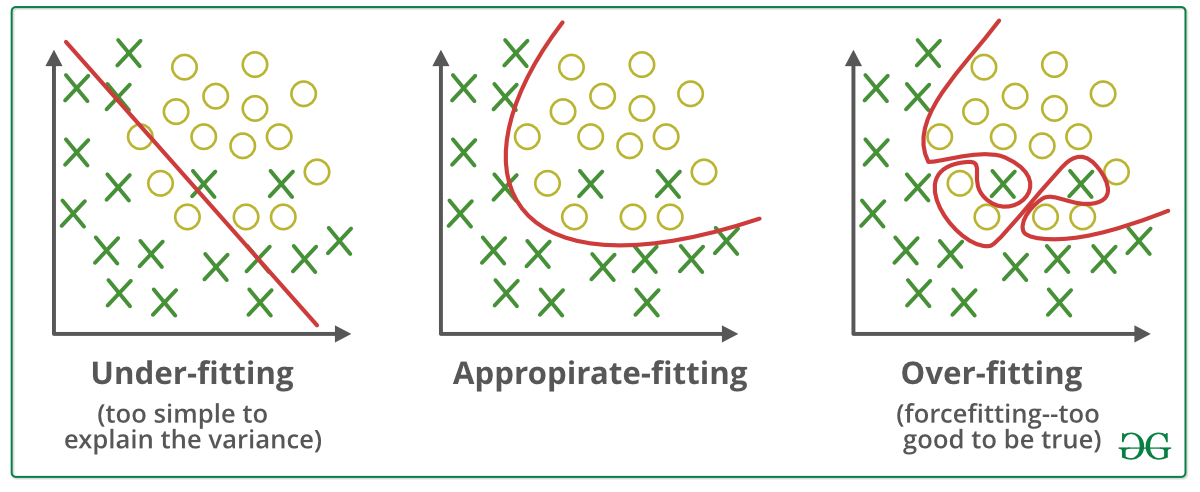
\includegraphics[width=0.7\linewidth]{images/overfitting_2}
		\caption{نمودار کم‌برازش در مقابل تعادل و بیش‌برازش}
		\label{fig:overfitting2}
	\end{figure}
	
	
\end{itemize}

برای کنترل این پدیده‌ها، می‌توان از روش‌هایی مانند استفاده از داده‌های اعتبارسنجی برای ارزیابی تعمیم‌پذیری، اعمال منظم‌سازی (مانند منظم‌سازی \(L2\) در رگرسیون ریج) برای کاهش پیچیدگی مدل، و انتخاب بهینه پیچیدگی مدل با تکنیک‌هایی مانند اعتبارسنجی متقاطع استفاده کرد. این رویکردها به تعادل بین دقت و تعمیم‌پذیری کمک می‌کنند و از افت عملکرد مدل در شرایط واقعی جلوگیری می‌نمایند.

\section{اعتبارسنجی متقاطع}

برای ارزیابی پایدار مدل‌ها، از روش اعتبارسنجی متقاطع استفاده می‌شود. در اعتبارسنجی \(k\)-بخشی، داده‌ها به \(k\) بخش مساوی تقسیم شده و هر بار یک بخش برای آزمون و باقی برای آموزش استفاده می‌شوند. میانگین عملکرد تمام تکرارها به‌عنوان عملکرد نهایی مدل گزارش می‌شود.

\section{روش نزول گرادیان}

\subsection[تابع هزینه چیست؟]{تابع هزینه\LTRfootnote{Cost Function} چیست؟}
تابع هزینه معیاری است که اختلاف بین خروجی پیش‌بینی‌شده توسط مدل و مقدار واقعی داده‌ها را اندازه‌گیری می‌کند. هدف اصلی، کمینه کردن این تابع است تا پارامترهای بهینه یافت شوند. برای رگرسیون خطی، تابع هزینه معمولاً میانگین مربعات خطاها تعریف می‌شود:
\[
J(\theta) = \frac{1}{m} \sum_{i=1}^{m} (h_\theta(x_i) - y_i)^2
\]
که در آن \(J(\theta)\) تابع هزینه، \(h_\theta(x_i)\) پیش‌بینی مدل، \(y_i\) مقدار واقعی، و \(m\) تعداد نمونه‌هاست.

\subsection{نزول گرادیان چیست؟}
نزول گرادیان یک الگوریتم بهینه‌سازی است که با تنظیم پارامترها در جهت مخالف گرادیان تابع هزینه، به کمینه آن می‌رسد. این روش مانند حرکت به سمت پایین‌ترین نقطه دره‌ای است که با محاسبه شیب تابع انجام می‌شود. این الگوریتم پایه‌ای برای آموزش مدل‌هایی مانند شبکه‌های عصبی است.

\subsection{نحوه کار نزول گرادیان چگونه است؟}
نزول گرادیان با محاسبه گرادیان تابع هزینه در نقطه فعلی آغاز می‌شود. پارامترها با فرمول زیر به‌روزرسانی می‌شوند:
\[
\theta_j := \theta_j - \alpha \frac{\partial J(\theta)}{\partial \theta_j}
\]
که در آن \(\theta_j\) پارامترها، \(\alpha\) نرخ یادگیری، و \(\frac{\partial J(\theta)}{\partial \theta_j}\) گرادیان تابع هزینه نسبت به پارامتر \(j\) است. این فرآیند تکراری است تا تابع هزینه به کمینه برسد. 

\begin{figure}[h]
	\centering
	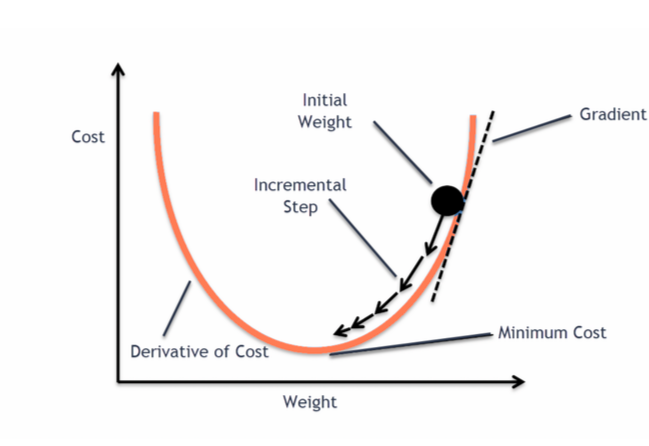
\includegraphics[width=0.7\linewidth]{images/gradient_process.png}
	\caption{نحوه کار نزول گرادیان در بهینه‌سازی}
	\label{fig:gradient_descent_process}
\end{figure}

\subsection[آلفا - نرخ یادگیری]{آلفا - نرخ یادگیری\LTRfootnote{Learning rate}}
نرخ یادگیری (\(\alpha\)) اندازه قدم‌ها در هر تکرار است. اگر \(\alpha\) بزرگ باشد، مدل ممکن است از کمینه عبور کند؛ اگر کوچک باشد، فرآیند کند می‌شود. فرمول به‌روزرسانی با نرخ یادگیری نشان می‌دهد که تعادل آن حیاتی است:
\[
\theta_{new} = \theta_{old} - \alpha \cdot \nabla J(\theta)
\]
تصویر \ref{fig:learning_rate} تأثیر نرخ‌های مختلف را با نمودار مقایسه می‌کند.

\begin{figure}[h]
	\centering
	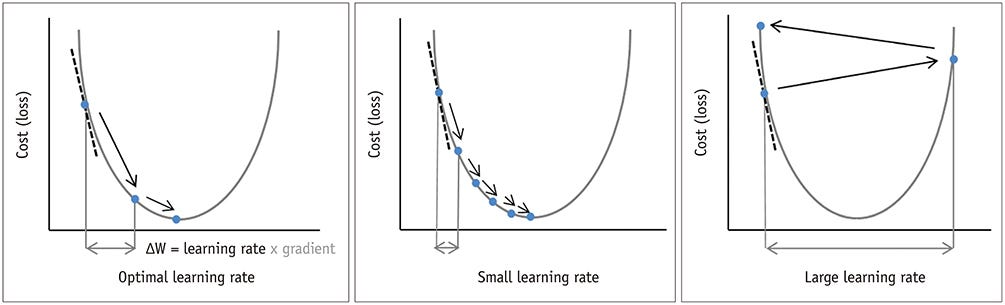
\includegraphics[width=0.7\linewidth]{images/learning_rate.jpg}
	\caption{تأثیر نرخ یادگیری بر فرآیند بهینه‌سازی}
	\label{fig:learning_rate}
\end{figure}

\subsection{کمینه‌های محلی}
کمینه‌های محلی نقاطی هستند که تابع هزینه در آن‌ها کاهش می‌یابد اما کمینه سراسری نیستند. مدل ممکن است در این نقاط گیر کند، به‌ویژه در توابع غیرخطی. تصویر \ref{fig:local_minima} این وضعیت را نشان می‌دهد.

\begin{figure}[h]
	\centering
	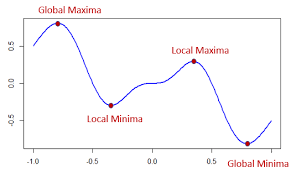
\includegraphics[width=0.7\linewidth]{images/local_minima.png}
	\caption{کمینه‌های محلی در تابع هزینه}
	\label{fig:local_minima}
\end{figure}

\subsection{مزایا و معایب}
نزول گرادیان دارای مزایای قابل‌توجهی است که از جمله آن‌ها می‌توان به سرعت بالا در بهینه‌سازی به‌ویژه در نسخه‌های کوچک‌دسته‌ای\LTRfootnote{Mini-Batch} برای داده‌های بزرگ اشاره کرد. این الگوریتم همچنین انعطاف‌پذیری بالایی دارد و می‌تواند برای انواع مدل‌ها مانند رگرسیون و شبکه‌های عصبی به‌کار رود، همچنین با تنظیم مناسب پارامترها امکان استفاده در مسائل پیچیده را فراهم می‌کند. با این حال، این روش با معایبی نیز همراه است؛ حساسیت به نرخ یادگیری نامناسب می‌تواند منجر به همگرایی ناقص شود و خطر به دام افتادن در کمینه‌های محلی در توابع غیرخطی وجود دارد. علاوه بر این، نیاز به محاسبات تکراری زیاد برای داده‌های بزرگ، این الگوریتم را در برخی موارد چالش‌برانگیز می‌کند.

\subsection*{مقایسه انواع روش‌های نزول گرادیان}
انواع مختلف نزول گرادیان، از جمله نزول گرادیان ساده\LTRfootnote{Batch Gradient Descent(BGD)}، نزول گرادیان تصادفی\LTRfootnote{Stochastic Gradient Descent(SGD)}، و نزول گرادیان کوچک‌دسته‌ای\LTRfootnote{Mini-Batch Gradient Descent}، هر یک ویژگی‌ها و کاربردهای خاص خود را دارند. جدول زیر این روش‌ها را از نظر نحوه محاسبه گرادیان، سرعت، دقت، و کاربردها مقایسه می‌کند:

\begin{table}[H]
	\centering
	\caption{مقایسه انواع روش‌های نزول گرادیان}
	\label{tab:gradient_descent_types}
	\begin{tabular}{|p{4cm}|p{3.5cm}|p{3.5cm}|p{3.5cm}|}
		\hline
		\textbf{ویژگی / روش} & \textbf{گرادیان ساده} & \textbf{گرادیان تصادفی} & \textbf{گرادیان مینی بچ} \\
		\hline
		واحد به‌روزرسانی پارامترها & کل مجموعه‌داده & یک نمونه تصادفی & دسته‌های کوچک \\
		\hline
		سرعت همگرایی & پایدار ولی کند & سریع ولی پرنوسان & تعادل میان سرعت و پایداری \\
		\hline
		نیاز حافظه & بالا & کم & متوسط \\
		\hline
		احتمال گیر کردن در مینیمم محلی & بیشتر & کمتر به‌دلیل نویز تصادفی & کمتر \\
		\hline
		مناسب برای داده‌های بزرگ & خیر & بله & بله \\
		\hline
		نوسان در مسیر گرادیان & ندارد & زیاد & کنترل‌شده \\
		\hline
		پیاده‌سازی ساده & بله & بله & نسبتاً پیچیده‌تر \\
		\hline
	\end{tabular}
\end{table}


\section[ناخالصی جینی]{ناخالصی جینی\LTRfootnote{Gini Impurity}}

یکی از معیارهای رایج برای سنجش کیفیت تقسیم داده‌ها در مدل‌های مبتنی بر درخت، ناخالصی جینی است. این معیار برای مسائل \textbf{دسته‌بندی}\LTRfootnote{Classification} به‌کار می‌رود و میزان اختلاط یا عدم خلوص نمونه‌های موجود در یک گره را اندازه‌گیری می‌کند.

اگر در یک گره خاص، نسبت نمونه‌های متعلق به دسته $k$ام برابر با $p_k$ باشد، مقدار ناخالصی جینی برای آن گره از رابطه زیر محاسبه می‌شود:
\[
\text{Gini} = 1 - \sum_{k=1}^{K} p_k^2
\]

که در آن:

\begin{itemize}
	\item $K$ تعداد کل دسته‌های ممکن است.
	\item $p_k$ احتمال حضور داده در دسته $k$ام در آن گره است.
\end{itemize}

مقدار این معیار همیشه بین ۰ و ۱ قرار دارد. اگر تمام نمونه‌های یک گره متعلق به یک دسته باشند، مقدار ناخالصی برابر با صفر خواهد بود که نشان‌دهنده خالص بودن گره است. هرچه توزیع نمونه‌ها در گره یکنواخت‌تر باشد (یعنی بین چند دسته پخش شده باشند)، مقدار ناخالصی افزایش می‌یابد.

در هنگام ساخت درخت، برای هر تقسیم ممکن، مقدار ناخالصی گره‌های حاصل از تقسیم محاسبه می‌شود و تقسیماتی انتخاب می‌شوند که ناخالصی کلی را کاهش دهند.

\section[اطلاعات کسب شده]{اطلاعات کسب شده\LTRfootnote{Information Gain}}

یکی دیگر از معیارهای متداول برای ارزیابی کیفیت تقسیم در درخت‌های تصمیم، اطلاعات کسب شده است که بر پایه مفهوم \textbf{آنتروپی}\LTRfootnote{Entropy} تعریف می‌شود. این معیار نیز معمولاً در مسائل دسته‌بندی کاربرد دارد.

آنتروپی یک گره به‌صورت زیر تعریف می‌شود:
\[
\text{Entropy} = - \sum_{k=1}^{K} p_k \log_2(p_k)
\]
که در آن:

\begin{itemize}
	\item $K$ تعداد دسته‌ها است.
	\item $p_k$ احتمال حضور یک نمونه در دسته $k$ام در آن گره است.
\end{itemize}

آنتروپی بیانگر میزان بی‌نظمی یا عدم قطعیت درون گره است. هرچه نمونه‌های یک گره به دسته‌های مختلف تعلق داشته باشند، مقدار آنتروپی بیشتر خواهد بود.

اطلاعات کسب شده برای یک تقسیم خاص برابر است با:
\[
\text{Information Gain} = \text{Entropy}_{\text{پیش از تقسیم}} - \sum_{i} \frac{n_i}{n} \cdot \text{Entropy}_i
\]
که در آن:
\begin{itemize}
	\item $n$ تعداد کل نمونه‌های گره مادر است.
	\item $n_i$ تعداد نمونه‌های هر گره فرزند پس از تقسیم است.
	\item $\text{Entropy}_i$ آنتروپی گره $i$ام است.
\end{itemize}

هدف الگوریتم در ساخت درخت، انتخاب تقسیم‌هایی است که بیشترین \textbf{کاهش آنتروپی} و در نتیجه بیشترین کسب اطلاعات را ایجاد کنند.


\section{مدل‌های مورد استفاده}

در این پژوهش از چندین مدل یادگیری ماشین برای پیش‌بینی مقدار اولین رکورد شیردهی گاو استفاده شده است. در ادامه، هر یک از این مدل‌ها با جزئیات بیشتری از نظر سازوکار ریاضی و نحوه عملکرد معرفی می‌گردند.

\subsection[رگرسیون ریج]{رگرسیون ریج\LTRfootnote{Ridge Regression}}

یکی از چالش‌های رایج در مدل‌سازی رگرسیون خطی، هم‌خطی چندگانه\LTRfootnote{Multicollinearity} میان ویژگی‌ها و همچنین بیش‌برازش مدل به داده‌های آموزشی است. روش رگرسیون ریج که با عنوان رگرسیون خطی با منظم‌سازی \(L2\) \LTRfootnote{L2-Regularized Linear Regression} نیز شناخته می‌شود، برای کاهش این مشکلات ارائه شده است.

در مدل رگرسیون خطی معمولی، هدف یافتن بردار ضرایب $\boldsymbol{w}$ است به‌گونه‌ای که مجموع مجذورات خطاهای مدل بر داده‌های آموزشی حداقل شود:
\[
\min_{\boldsymbol{w}} \sum_{i=1}^{n} \left( y_i - \boldsymbol{w}^\top \boldsymbol{x}_i \right)^2
\]

اما در رگرسیون ریج، برای جلوگیری از بزرگ شدن بیش از حد ضرایب، یک جمله‌ی جریمه (پنالتی) به تابع هدف افزوده می‌شود:
\[
\min_{\boldsymbol{w}} \sum_{i=1}^{n} \left( y_i - \boldsymbol{w}^\top \boldsymbol{x}_i \right)^2 + \lambda \| \boldsymbol{w} \|_2^2
\]
که در آن:
\begin{itemize}
	\item $\boldsymbol{x}_i$ بردار ویژگی‌های نمونه‌ی $i$ام است.
	\item $y_i$ خروجی یا مقدار هدف برای نمونه‌ی $i$ام است.
	\item $\boldsymbol{w}$ بردار ضرایب مدل است.
	\item $\lambda \geq 0$ پارامتر منظم‌سازی است که شدت جریمه را کنترل می‌کند.
	\item $\| \boldsymbol{w} \|_2^2 = \sum_{j=1}^{p} w_j^2$ مربع نرم \(L2\)  ضرایب است.
\end{itemize}

هنگامی که $\lambda = 0$، مدل معادل با رگرسیون خطی معمولی خواهد بود. با افزایش $\lambda$، مدل به سمت کاهش اندازه ضرایب و در نتیجه جلوگیری از پیچیدگی بیش‌ از حد گرایش پیدا می‌کند. در رگرسیون ریج همه ضرایب کوچک ولی غیرصفر باقی می‌مانند. بنابراین این روش زمانی مناسب است که انتظار می‌رود تمامی ویژگی‌ها تا حدودی در پیش‌بینی مؤثر باشند.

\vspace{0.5em}
\subsection*{حل با استفاده از نزول گرادیان}

در مسائل با داده‌های پرتعداد یا تعداد ویژگی‌های زیاد، حل تحلیلی مدل ممکن است دشوار یا ناکارآمد باشد. در این موارد، می‌توان از الگوریتم نزول گرادیان برای یافتن ضرایب استفاده کرد.

تابع هزینه در این حالت به شکل زیر تعریف می‌شود:
\[
J(\boldsymbol{w}) = \frac{1}{n} \sum_{i=1}^{n} \left( y_i - \boldsymbol{w}^\top \boldsymbol{x}_i \right)^2 + \lambda \| \boldsymbol{w} \|_2^2
\]
در هر تکرار الگوریتم، بردار ضرایب $\boldsymbol{w}$ با استفاده از گرادیان تابع هزینه به‌روزرسانی می‌شود:
\[
\boldsymbol{w} \leftarrow \boldsymbol{w} - \alpha \nabla J(\boldsymbol{w})
\]
که در آن $\alpha$ نرخ یادگیری و گرادیان تابع هزینه به‌صورت برداری برابر است با:
\[
\nabla J(\boldsymbol{w}) = -\frac{2}{n} \boldsymbol{X}^\top \left( \boldsymbol{y} - \boldsymbol{Xw} \right) + 2\lambda \boldsymbol{w}
\]
در نهایت، مدل رگرسیون ریج برای پیش‌بینی خروجی جدید به‌صورت زیر نوشته می‌شود:
\[
\hat{y} = \boldsymbol{w}^\top \boldsymbol{x} + b
\]
که در آن $b$ مقدار بایاس (اختیاری) و $\hat{y}$ مقدار پیش‌بینی‌شده است.

\subsection[درخت تصمیم]{درخت تصمیم\LTRfootnote{Decision Tree}}

درخت تصمیم یکی از مدل‌های پایه‌ای، ساده و در عین حال مؤثر در یادگیری ماشین است که برای حل مسائل دسته‌بندی و رگرسیون به‌کار می‌رود. این مدل ساختاری درختی دارد که از تقسیم متوالی داده‌ها بر اساس ویژگی‌های آن‌ها تشکیل می‌شود.

هر درخت تصمیم از مجموعه‌ای از \textbf{گره‌های تصمیم\LTRfootnote{Decision Nodes}} و \textbf{برگ‌ها\LTRfootnote{Leaves}} تشکیل شده است. در گره‌های تصمیم، بر اساس یک شرط مشخص (مثلاً "آیا ویژگی $x_j$ از مقدار معینی کمتر است؟") داده‌ها به دو شاخه تقسیم می‌شوند و این روند تا رسیدن به گره‌های نهایی (برگ‌ها) ادامه می‌یابد. هر برگ بیانگر خروجی نهایی مدل برای داده‌هایی است که به آن گره رسیده‌اند.

\subsection*{فرایند ساخت درخت}

مراحل کلی آموزش یک درخت تصمیم عبارت‌اند از:

\begin{enumerate}
	\item انتخاب بهترین ویژگی و مقدار آستانه برای تقسیم داده‌ها در هر گره. این انتخاب بر اساس معیارهایی مانند:
	\begin{itemize}
		\item ناخالصی جینی
		\item اطلاعات کسب شده(بر اساس آنتروپی)
		\item میانگین مربعات خطا (برای مسائل رگرسیون)
	\end{itemize}
	صورت می‌گیرد.
	\item تقسیم داده‌ها به دو زیرمجموعه بر اساس ویژگی انتخاب‌شده.
	\item تکرار مرحله بالا به‌صورت بازگشتی تا زمانی که یکی از شرایط توقف برقرار شود:
	\begin{itemize}
		\item رسیدن به حداکثر عمق درخت
		\item تعداد نمونه‌های گره کمتر از مقدار آستانه
		\item خالص بودن داده‌های گره (برای مسائل رده‌بندی)
	\end{itemize}
\end{enumerate}

درخت تصمیم به دلیل سادگی و تفسیرپذیری خود برجسته است، زیرا خروجی آن به‌صورت سلسله‌مراتبی و قابل فهم برای انسان ارائه می‌شود. این مدل همچنین نیازی به نرمال‌سازی داده‌ها ندارد و نسبت به مقیاس ویژگی‌ها حساس نیست. از دیگر مزایای آن، پشتیبانی از ویژگی‌های عددی و طبقه‌ای است که امکان استفاده از هم داده‌های پیوسته و هم داده‌های گسسته را فراهم می‌سازد.

\subsection*{مدل ریاضی برای رگرسیون}

در مسائل رگرسیون، مقدار خروجی هر برگ به‌صورت میانگین مقادیر هدف داده‌هایی که به آن گره رسیده‌اند تعریف می‌شود. بنابراین مدل کلی برای پیش‌بینی $\hat{y}$ به شکل زیر است:
\[
\hat{y} = \frac{1}{|L(x)|} \sum_{i \in L(x)} y_i
\]
که در آن:
\begin{itemize}
	\item $L(x)$ مجموعه نمونه‌هایی است که در داده‌های آموزشی به همان برگ که $x$ به آن تعلق می‌گیرد، رسیده‌اند.
	\item $y_i$ مقدار هدف برای نمونه $i$ام است.
\end{itemize}

این مدل اگرچه ساده است، اما به‌تنهایی ممکن است دچار بیش‌برازش شود، و به همین دلیل در الگوریتم‌هایی مانند جنگل تصادفی یا افزایش گرادیان افراطی به‌صورت ترکیبی از چند درخت مورد استفاده قرار می‌گیرد.



\subsection[جنگل تصادفی]{جنگل تصادفی\LTRfootnote{Random Forest}}

جنگل تصادفی یکی از مدل‌های قدرتمند و پرکاربرد در یادگیری ماشین است که در مسائل دسته‌بندی و رگرسیون استفاده می‌شود. این مدل بر پایه الگوریتم درخت تصمیم ساخته شده و با ترکیب تعداد زیادی از درخت‌های تصمیم، دقت و پایداری مدل را افزایش می‌دهد.

مدل جنگل تصادفی از رویکرد \textbf{یادگیری تجمعی\LTRfootnote{Ensemble Learning}} بهره می‌برد؛ به این معنا که به‌جای تکیه بر یک مدل منفرد، مجموعه‌ای از مدل‌ها به‌طور موازی آموزش می‌بینند و خروجی نهایی بر اساس تجمیع تصمیم آن‌ها به‌دست می‌آید.

\subsection*{مراحل ساخت مدل}

الگوریتم جنگل تصادفی شامل مراحل زیر است:

\begin{enumerate}
	\item با استفاده از روش نمونه‌گیری تکراری\LTRfootnote{Bootstrap Sampling} چندین نمونه تصادفی (با تکرار) از داده‌های آموزشی گرفته می‌شود.
	\item برای هر نمونه، یک درخت تصمیم مستقل ساخته می‌شود.
	\item در هر گره از هر درخت، به‌جای بررسی تمام ویژگی‌ها، تنها یک زیرمجموعه تصادفی از ویژگی‌ها برای تقسیم گره انتخاب می‌شود. این کار موجب تنوع بیشتر میان درخت‌ها می‌شود.
	\item برای پیش‌بینی یک نمونه جدید، خروجی تمام درخت‌ها محاسبه می‌شود:
	\begin{itemize}
		\item در رگرسیون: میانگین خروجی درخت‌ها به‌عنوان پیش‌بینی نهایی انتخاب می‌شود.
		\item در دسته‌بندی: از رای‌گیری اکثریت میان خروجی درخت‌ها استفاده می‌شود.
	\end{itemize}
\end{enumerate}

جنگل تصادفی با ترکیب چندین درختی که روی داده‌ها و ویژگی‌های متفاوت آموزش دیده‌اند، به کاهش بیش‌برازش کمک می‌کند و از این طریق مدل نهایی را از وابستگی بیش از حد به داده‌های آموزشی محافظت می‌کند. همچنین، این مدل از پایداری بالایی برخوردار است، زیرا حساسیت آن به داده‌های پرت یا نویز به‌طور قابل‌توجهی کاهش می‌یابد. از دیگر مزایای آن، قابلیت سنجش اهمیت ویژگی‌هاست که امکان ارزیابی میزان تأثیر هر ویژگی بر نتیجه نهایی را فراهم می‌سازد.

\subsection*{مدل ریاضی برای رگرسیون}

فرض کنید $T_1(x), T_2(x), \dots, T_K(x)$ خروجی‌های $K$ درخت تصمیم آموزش‌دیده باشند. در این صورت، پیش‌بینی نهایی مدل جنگل تصادفی برای ورودی $x$ در مسئله رگرسیون به‌صورت زیر خواهد بود:
\[
\hat{y} = \frac{1}{K} \sum_{k=1}^{K} T_k(x)
\]
که در آن $\hat{y}$ خروجی پیش‌بینی‌شده و $K$ تعداد درخت‌ها در جنگل است.


\subsection[رگرسیون بردار پشتیبان]{رگرسیون بردار پشتیبان\LTRfootnote{Support Vector Regression(SVR)}}


رگرسیون بردار پشتیبان یکی از انواع الگوریتم‌های ماشین بردار پشتیبان\LTRfootnote{Support Vector Machine (SVM)} است و به‌طور رایج برای تحلیل‌های رگرسیونی مورد استفاده قرار می‌گیرد. الگوریتم‌های ماشین بردار پشتیبان، روش‌هایی قدرتمند در حوزه یادگیری با ناظر هستند که در اصل برای حل مسائل \textbf{دسته‌بندی} طراحی شده‌اند.

هدف الگوریتم ماشین بردار پشتیبان، یافتن \textbf{ابرصفحه‌ای}\LTRfootnote{Hyperplane} بهینه است که به بهترین شکل ممکن دو دسته را در فضای ویژگی از هم جدا کند. منظور از ابرصفحه، یک زیرفضای تخت با بُعد \(p-1\) در فضای \(p\)-بعدی است که \(p\) برابر با تعداد ویژگی‌های ورودی می‌باشد. ابرصفحه بهینه، صفحه‌ای است که \textbf{حاشیه}\LTRfootnote{Margin} را حداکثر می‌کند. منظور از حاشیه، فاصله بین ابرصفحه و نزدیک‌ترین نقاط از هر دسته است که به آن‌ها \textbf{بردارهای پشتیبان}\LTRfootnote{Support Vectors} گفته می‌شود.

رگرسیون بردار پشتیبان نیز همچون نسخه دسته‌بندی، بر مفهوم ابرصفحه و حاشیه تکیه دارد، اما تعریف این مفاهیم در آن متفاوت است. در رگرسیون بردار پشتیبان، حاشیه به‌صورت \textbf{ناحیه تحمل خطا}\LTRfootnote{$\varepsilon$-insensitive tube} تعریف می‌شود. این ناحیه، یک نوار اطراف ابرصفحه را در نظر می‌گیرد که مقادیر خروجی تا میزان \(\varepsilon\) می‌توانند از آن انحراف داشته باشند بدون اینکه به‌عنوان خطا محسوب شوند.

ابرصفحه در این مدل، بهترین برازش ممکن برای داده‌هایی است که درون این نوار قرار دارند. تفاوت اصلی میان مدل دسته‌بندی و رگرسیون در این است که در دسته‌بندی، هدف جداسازی داده‌ها است، اما در رگرسیون، هدف برازش داده‌ها در ناحیه‌ای مجاز از خطا است.

\begin{figure}[h]
	\centering
	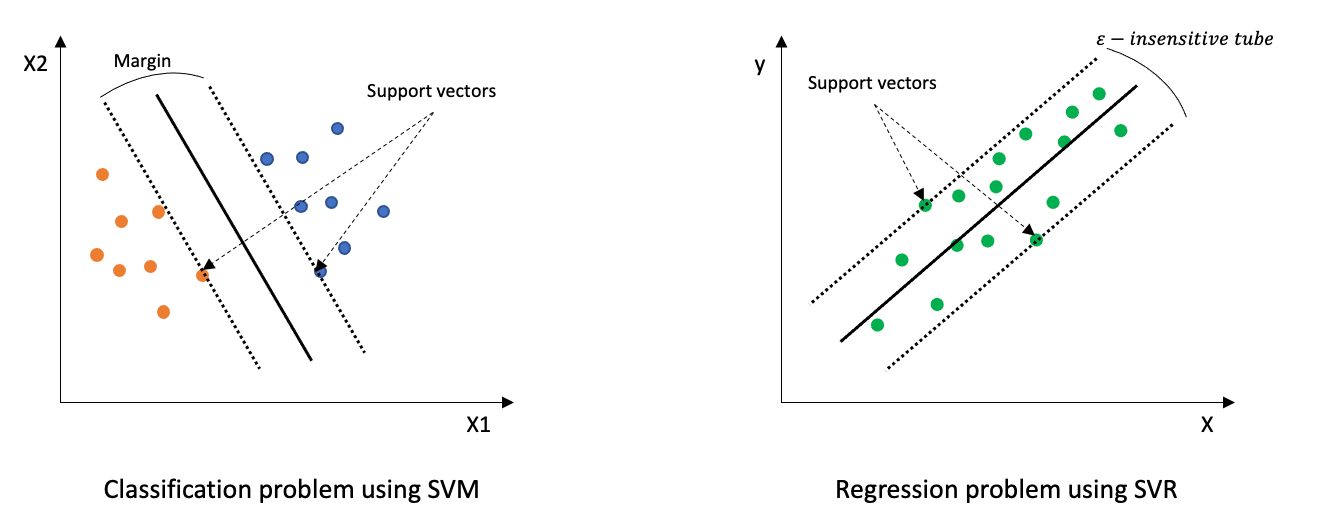
\includegraphics[width=0.7\linewidth]{images/SVR_SVM}
	\caption{تفاوت رگرسیون بردار پشتیبان و ماشین بردار پشتیبان}
	\label{fig:svrsvm}
\end{figure}

\subsection*{مبنای نظری مدل رگرسیون بردار پشتیبان}

در مدل رگرسیون بردار پشتیبان، هدف یافتن بهترین تابع برازش است که بتواند مقدار متغیر هدف را به‌درستی پیش‌بینی کرده و هم‌زمان از نظر پیچیدگی نیز ساده باقی بماند تا از بیش‌برازش جلوگیری شود. برای تحقق این هدف، ناحیه‌ای به نام \textbf{نوار تحمل‌پذیر} پیرامون ابرصفحه تعریف می‌شود که اجازه می‌دهد مقدار پیش‌بینی‌شده تا حدی (\(\varepsilon\)) با مقدار واقعی تفاوت داشته باشد. این ناحیه سبب ایجاد تعادلی میان سادگی مدل و توانایی تعمیم آن به داده‌های جدید می‌شود.

این مدل به‌صورت یک \textbf{مسئله بهینه‌سازی محدب}\LTRfootnote{Convex Optimization Problem} فرموله می‌شود. هدف از این بهینه‌سازی، یافتن تابعی به صورت \(f(x)\) است که تا حد ممکن \textbf{صاف}\LTRfootnote{Flat} باشد و بیشینه انحراف آن از مقدار واقعی خروجی، برای تمامی داده‌های آموزشی، بیشتر از \(\varepsilon\) نباشد.

صاف بودن تابع بدین معناست که حساسیت آن نسبت به تغییرات کوچک در ورودی پایین باشد؛ در نتیجه خطر بیش‌برازش کاهش می‌یابد. در حالت تابع خطی، صاف بودن به این معناست که مقدار بردار وزن‌ها\LTRfootnote{Weight Vector} (\textit{w}) در تابع \(f(x) = wx + b\) کوچک باشد.

\subsection*{مدل ریاضی رگرسیون بردار پشتیبان}

مدل رگرسیون بردار پشتیبان را می‌توان به‌صورت یک مسئله بهینه‌سازی محدب فرموله کرد که در آن هدف، یافتن تابعی است که تا حد امکان صاف باشد و از مقادیر خروجی واقعی داده‌ها، بیش از مقدار \(\varepsilon\) منحرف نشود.

تابع هدف برای این مدل به‌صورت زیر تعریف می‌شود:
\[
\min_{w, b, \xi_i, \xi_i^*} \ \frac{1}{2} \|w\|^2 + C \sum_{i=1}^{n} (\xi_i + \xi_i^*)
\]
که در آن:
\begin{itemize}
	\item \(w\) بردار وزن‌ها در تابع خطی است.
	\item \(b\) عرض از مبدأ است.
	\item \(C\) یک \textbf{پارامتر تنظیم}\LTRfootnote{Regularization Parameter} است که بین پیچیدگی مدل و میزان خطا تعادل برقرار می‌کند.
	\item \(\xi_i\) و \(\xi_i^*\) متغیرهای افزایشی هستند که میزان نقض ناحیه \(\varepsilon\) را در هر طرف ابرصفحه اندازه‌گیری می‌کنند.
\end{itemize}

این بهینه‌سازی با رعایت محدودیت‌های زیر انجام می‌شود:
\[
\begin{cases}
	y_i - (w^\top x_i + b) \le \varepsilon + \xi_i \\
	(w^\top x_i + b) - y_i \le \varepsilon + \xi_i^* \\
	\xi_i \ge 0, \quad \xi_i^* \ge 0
\end{cases}
\]
که در آن:
\begin{itemize}
	\item \(x_i\) نمونه ورودی \(i\)ام،
	\item و \(y_i\) مقدار خروجی متناظر با آن است.
\end{itemize}

هدف از کمینه‌سازی عبارت \(\frac{1}{2} \|w\|^2\)، تولید تابعی است که تا حد ممکن صاف باشد. در عین حال، جمله \(\sum (\xi_i + \xi_i^*)\) میزان خطاهای خارج از ناحیه \(\varepsilon\) را اندازه می‌گیرد، و پارامتر \(C\) نقش وزنی برای این خطاها ایفا می‌کند.

ترکیب این دو بخش، مدلی را می‌سازد که به خوبی تعادلی میان دقت، توانایی تعمیم و جلوگیری از پیچیدگی بیش‌ازحد ایجاد می‌کند.

\begin{figure}[H]
	\centering
	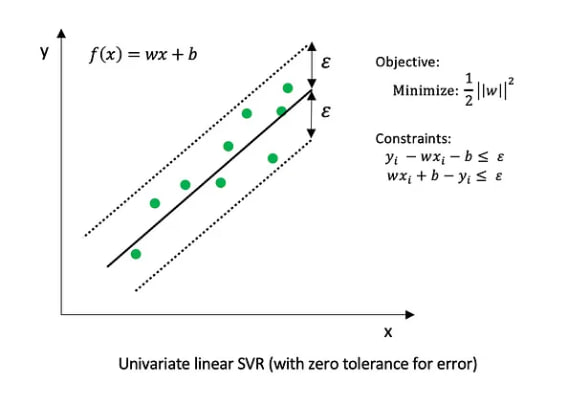
\includegraphics[width=0.7\linewidth]{images/svr_formula1}
	\caption{مدل ریاضی و نمودار رگرسیون بردار پشتیبان }
	\label{fig:svrformula1}
\end{figure}


در برخی موارد، ممکن است مسئله بهینه‌سازی قابل حل نباشد، یا بخواهیم اجازه دهیم مقدار کمی خطا در مدل وجود داشته باشد. برای این منظور، از \textbf{متغیرهای افزایشی}\LTRfootnote{Slack Variables} استفاده می‌شود. این متغیرها مربوط به داده‌هایی هستند که خارج از ناحیه تحمل‌پذیر \(\varepsilon\) قرار می‌گیرند. فاصله این نقاط از مرز ناحیه \(\varepsilon\) با نماد \(\xi\) نمایش داده می‌شود.

برای برقراری تعادل میان پیچیدگی مدل (یعنی صاف بودن تابع \(f(x)\)) و مجموع انحراف‌های فراتر از ناحیه \(\varepsilon\)، از یک پارامتر منظم‌ساز با نماد \(C > 0\) استفاده می‌شود. میزان قدرت این منظم‌سازی رابطه معکوس با مقدار \(C\) دارد؛ یعنی هرچه مقدار \(C\) بزرگ‌تر باشد، مدل تمایل بیشتری به کاهش خطاهای خارج از ناحیه \(\varepsilon\) خواهد داشت و در مقابل، صاف بودن تابع را کمتر در نظر می‌گیرد.

مدل رگرسیون بردار پشتیبان، برای نمونه‌هایی که درون ناحیه \(\varepsilon\) قرار دارند، خطای پیش‌بینی برابر با صفر در نظر می‌گیرد؛ اما برای داده‌هایی که بیرون از این ناحیه هستند (یعنی متغیرهای افزایشی)، جریمه‌ای متناسب با مقدار \(\xi\) اعمال می‌کند.

این ویژگی رگرسیون بردار پشتیبان را قادر می‌سازد تا در مقایسه با مدل‌های رگرسیون معمولی، بهتر با پدیده بیش‌برازش مقابله کند.

\begin{figure}[H]
	\centering
	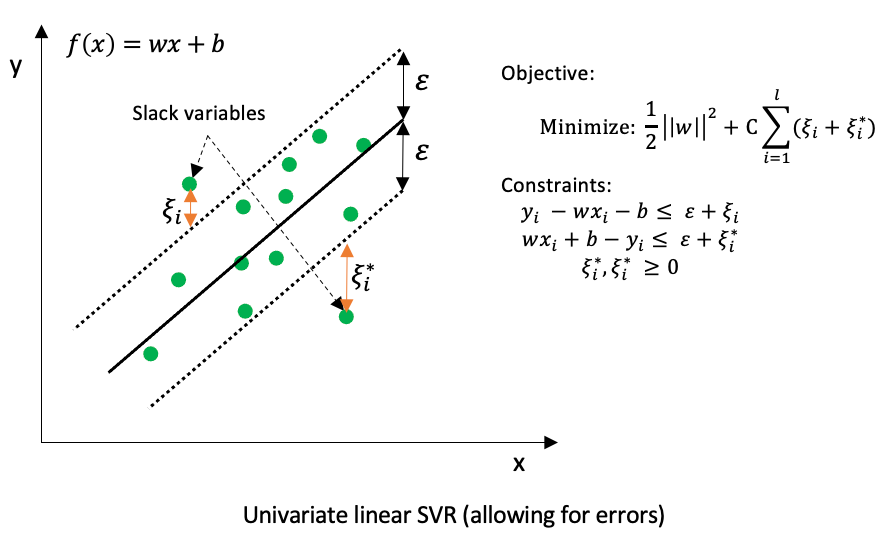
\includegraphics[width=0.7\linewidth]{images/SVR_FORMULA2}
	\caption{مدل ریاضی و نمودار رگرسیون بردار پشتیبان با متغیر های افزایشی}
	\label{fig:svrformula2}
\end{figure}

\subsection*{رگرسیون غیرخطی با استفاده از تابع هسته}

مدل رگرسیون بردار پشتیبان می‌تواند هم برای مسائل خطی و هم برای مسائل غیرخطی به‌کار رود. این قابلیت با استفاده از \textbf{تابع هسته}\LTRfootnote{Kernel Function} فراهم می‌شود. 

در شرایطی که داده‌ها به‌صورت غیرخطی از یکدیگر قابل تفکیک هستند، از تابع هسته برای نگاشت داده‌ها به یک فضای با ابعاد بالاتر استفاده می‌شود؛ به‌طوری‌که در آن فضا بتوان یک مسئله خطی (و در نتیجه رگرسیون خطی) را حل کرد. در واقع، تابع هسته اجازه می‌دهد بدون نیاز به محاسبه مستقیم نگاشت به فضای جدید، مدل رگرسیون به‌صورت غیرخطی رفتار کند.

در میان توابع هسته که در رگرسیون بردار پشتیبان مورد استفاده قرار می‌گیرند، چهار نوع متداول‌تر وجود دارد. نخست، \textbf{هسته خطی}\LTRfootnote{Linear Kernel} که ساده‌ترین نوع هسته است و معمولاً در مسائل با رابطه‌های تقریباً خطی میان متغیرها به‌کار می‌رود. دوم، \textbf{هسته چندجمله‌ای}\LTRfootnote{Polynomial Kernel} است که قادر به مدل‌سازی روابط غیرخطی از طریق ترکیب‌های چندجمله‌ای میان ویژگی‌ها می‌باشد. سوم، \textbf{هسته پایه شعاعی}\LTRfootnote{Radial Basis Function (RBF) Kernel} که قدرت بالایی در مدل‌سازی داده‌های پیچیده و غیرخطی دارد و از متداول‌ترین گزینه‌ها در مسائل مختلف یادگیری ماشین محسوب می‌شود. در نهایت، \textbf{هسته سیگموئید}\LTRfootnote{Sigmoid Kernel} وجود دارد که عملکردی مشابه نورون‌های شبکه عصبی دارد و در برخی کاربردهای خاص مورد استفاده قرار می‌گیرد.


انتخاب نوع هسته به ماهیت داده‌ها و رابطه میان ویژگی‌ها و متغیر هدف بستگی دارد. 

\begin{table}[H]
	\centering
	\caption{مقایسه انواع تابع‌های هسته در رگرسیون بردار پشتیبان}
	\label{tab:kernels}
		\begin{tabular}{|c|c|c|c|}
			\hline
			\textbf{نام هسته} & \textbf{فرمول ریاضی} & \textbf{پارامترهای قابل تنظیم} & \textbf{ویژگی‌ها و کاربردها} \\
			\hline
			خطی & $K(x,x') = x^\top x'$ & ندارد & ساده، سریع، مناسب برای داده‌هایی با رابطه تقریباً خطی \\
			\hline
			چندجمله‌ای & $K(x,x') = (x^\top x' + c)^d$ & $c$، $d$ & مناسب برای داده‌هایی با رابطه چندجمله‌ای، انعطاف‌پذیر \\
			\hline
			پایه شعاعی & $K(x,x') = \exp(-\gamma \|x - x'\|^2)$ & $\gamma$ & بسیار قدرتمند، مناسب برای داده‌های غیرخطی پیچیده \\
			\hline
			سیگموئید & $K(x,x') = \tanh(\alpha x^\top x' + c)$ & $\alpha$، $c$ & مشابه نورون در شبکه عصبی، حساس به پارامترها \\
			\hline
		\end{tabular}
\end{table}




\subsection[افزایش گرادیان افراطی]{افزایش گرادیان افراطی\LTRfootnote{Extreme Gradient Boosting(XGBoost)}}

مدل افزایش گرادیان افراطی، یکی از الگوریتم‌های \textbf{یادگیری با نظارت} محسوب می‌شود که برای حل مسائل رگرسیون و دسته‌بندی بسیار پرکاربرد است. 

این مدل بر پایه درخت تصمیم عمل می‌کند و از نوع \textbf{یادگیری تجمعی ترتیبی}\LTRfootnote{Sequential Ensemble Learning} محسوب می‌شود. این روش نیازی به مقیاس‌بندی ویژگی‌ها ندارد و نسبت به داده‌های پرت\LTRfootnote{Outliers} حساسیت کمی نشان می‌دهد. همچنین، به‌صورت پیش‌فرض قادر به مدیریت مقادیر گمشده\LTRfootnote{Missing Values} است.

\subsection*{مراحل اجرای مدل افزایش گرادیان افراطی}

\begin{enumerate}
	\item \textbf{پیش‌بینی اولیه}:  با انجام یک پیش‌بینی ساده روی داده‌های آموزشی آغاز می‌شود. این پیش‌بینی معمولاً میانگین مقدار متغیر هدف را در نظر می‌گیرد.
	
	\item \textbf{محاسبه خطا}: سپس باقی‌مانده‌ها (اختلاف بین مقدار واقعی و مقدار پیش‌بینی‌شده) محاسبه می‌شوند. این باقی‌مانده‌ها بیانگر خطاهای موجود در پیش‌بینی اولیه هستند.
	
	\item \textbf{ساخت اولین درخت تصمیم}: اولین درخت تصمیم در مجموعه مدل‌ها ساخته می‌شود. این درخت بر روی یادگیری همین باقی‌مانده‌ها متمرکز است و هدف آن کاهش مجموع خطاهاست. برای این منظور، درخت به‌دنبال یافتن بهترین نقاط تقسیم ویژگی‌ها برای کاهش بیشینه خطاها می‌گردد.
	
	\item \textbf{درخت‌های بعدی و اصلاح خطا}: در این مرحله، فرآیند \textbf{تقویت گرادیانی}\LTRfootnote{Gradient Boosting} به‌کار گرفته می‌شود. درخت جدید باقی‌مانده‌های به‌روز‌شده‌ای را هدف قرار می‌دهد که در پیش‌بینی مدل تجمعی (شامل همه درخت‌های قبلی) هنوز باقی مانده‌اند. هر درخت جدید به بهبود دقت مدل نهایی کمک می‌کند.
	
	\item \textbf{کمینه‌سازی تابع زیان}: در تمام مراحل، الگوریتم به‌طور پیوسته تابع زیان\LTRfootnote{Loss Function} را بهینه می‌کند. این تابع به‌صورت ریاضی اندازه می‌گیرد که پیش‌بینی‌های مدل تا چه میزان با مقادیر واقعی تطابق دارند. با کمینه‌سازی این تابع، مدل به‌سمت پیش‌بینی‌های دقیق‌تر هدایت می‌شود.
	
	\item \textbf{معیار توقف}: فرآیند افزودن درخت‌ها تا زمانی ادامه می‌یابد که یکی از شرایط توقف برقرار شود. این شرایط می‌تواند شامل: رسیدن به حداکثر تعداد درخت‌ها، کاهش کمتر از آستانهٔ مشخص در تابع زیان، یا دستیابی به سطح مشخصی از دقت باشد.
\end{enumerate}

\begin{figure}[H]
	\centering
	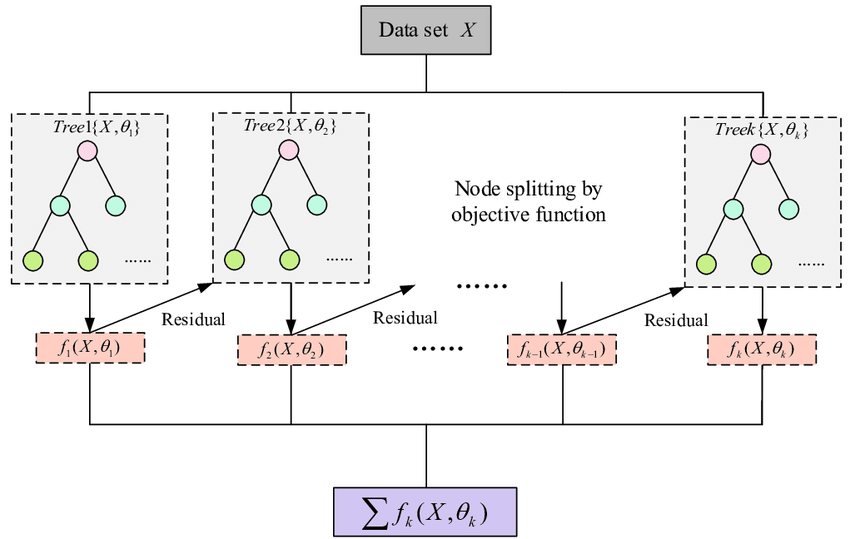
\includegraphics[width=0.7\linewidth]{images/xgboost}
	\caption{کارکر مدل افزایش گرادیان افراطی}
	\label{fig:xgboost}
\end{figure}


\subsection[تقویت دسته‌ای]{مدل تقویت دسته‌ای\LTRfootnote{Category Boosting(CatBoost)}}

در حوزهٔ یادگیری ماشین، روش‌های تقویت گرادیانی تحولی اساسی در حل مسائل رگرسیون و دسته‌بندی ایجاد کرده‌اند. در میان این روش‌ها، مدل تقویت دسته‌ای به‌عنوان الگوریتمی قدرتمند، کارا و منعطف شناخته می‌شود که توانایی پردازش مستقیم داده‌های دسته‌ای\LTRfootnote{Categorical Data} را دارد؛ بدون آن‌که به پیش‌پردازش پیچیده‌ای نیاز داشته باشد.

مدل تقویت دسته‌ای، کتابخانه‌ای متن‌باز می‌باشد. این الگوریتم به‌گونه‌ای طراحی شده که بتواند متغیرهای دسته‌ای را بدون نیاز به تبدیل آن‌ها به قالب عددی (مانند کدگذاری وان-هات\LTRfootnote{One-Hot Encoding} یا روش‌های مشابه) مستقیماً پردازش نماید. این ویژگی، فرآیند آماده‌سازی داده‌ها را ساده‌تر کرده و عملکرد مدل را بهبود می‌بخشد.

این مدل نیز بر پایهٔ اصل تقویت گرادیانی عمل می‌کند؛ بدین‌صورت که مدل به‌صورت مرحله‌ای ساخته می‌شود. الگوریتم با مدلی ساده آغاز می‌گردد و سپس به‌صورت افزایشی، مدل‌های جدیدی را اضافه می‌کند که هدف آن‌ها اصلاح خطاهای مدل‌های قبلی است. با این حال، تقویت دسته‌ای نوآوری‌های مهمی را نسبت به سایر الگوریتم‌های تقویت گرادیانی ارائه می‌دهد:

\vspace{0.3cm}
\textbf{پردازش ویژگی‌های دسته‌ای:}

این مدل برای تبدیل مقادیر دسته‌ای به مقادیر عددی از الگوریتمی نوآورانه بهره می‌گیرد که در آن ترتیب دسته‌ها بر اساس متغیر هدف تعیین می‌شود. این فرآیند با عنوان \textbf{آمار هدف}\LTRfootnote{Target Statistics} شناخته می‌شود و به کاهش بیش‌برازش کمک کرده و نمایشی دقیق‌تر از داده‌های دسته‌ای ارائه می‌دهد.

\vspace{0.3cm}
\textbf{تقویت ترتیبی:}

یکی از نوآوری‌های اصلی تقویت دسته‌ای، استفاده از سازوکار \textbf{تقویت ترتیبی}\LTRfootnote{Ordered Boosting} است. الگوریتم‌های تقویت گرادیانی سنتی ممکن است دچار \textbf{جابجایی پیش‌بینی}\LTRfootnote{Prediction Shift} شوند، چراکه داده‌های مورد استفاده برای آموزش و محاسبه گرادیان با هم هم‌پوشانی دارند. برای رفع این مشکل، تقویت دسته‌ای در هر تکرار از یک جایگشت تصادفی از مجموعه‌داده استفاده می‌کند و فقط داده‌های قبل از هر نمونه در آن جایگشت را برای آموزش به‌کار می‌گیرد. این روش، میزان بیش‌برازش را کاهش داده و پایداری مدل را افزایش می‌دهد.

\vspace{0.3cm}
\textbf{درخت‌های متقارن:}

تقویت دسته‌ای از درخت‌های متقارن\LTRfootnote{Symmetric Trees} به‌عنوان پیش‌بینی‌های پایه استفاده می‌کند. برخلاف روش‌های سنتی که درخت‌ها را به‌صورت عمقی یا بر اساس برگ‌ها گسترش می‌دهند، تقویت دسته‌ای درخت‌هایی می‌سازد که در آن تمامی گره‌های یک سطح از قاعدهٔ تصمیم‌گیری یکسانی پیروی می‌کنند. این ساختار موجب اجرای سریع‌تر و کاهش احتمال بیش‌برازش می‌گردد.

\subsection*{مراحل ساخت مدل تقویت دسته‌ای}

روند ساخت مدل تقویت دسته‌ای شامل مراحل زیر است:

\begin{enumerate}
	\item \textbf{آماده‌سازی داده‌ها:} این مدل توانایی پردازش هم‌زمان ویژگی‌های عددی و دسته‌ای را دارد. برای ویژگی‌های دسته‌ای از یک روش رمزگذاری نوین مبتنی بر آمار هدف استفاده می‌کند.
	\item \textbf{آموزش مدل:} مدل به‌صورت افزایشی آموزش داده می‌شود. در هر مرحله، درخت‌هایی افزوده می‌شوند که خطاهای مدل‌های قبلی را اصلاح می‌کنند. بهینه‌سازی مدل از طریق الگوریتمی مبتنی بر گرادیان برای کمینه‌سازی \textbf{تابع زیان} انجام می‌شود.
	\item \textbf{اعمال تقویت ترتیبی و درخت‌های متقارن:} این دو سازوکار به مدل کمک می‌کنند تا با کاهش بیش‌برازش، داده‌های دسته‌ای را به‌صورت مؤثر و دقیق مدیریت کند.
\end{enumerate}


\begin{figure}[H]
	\centering
	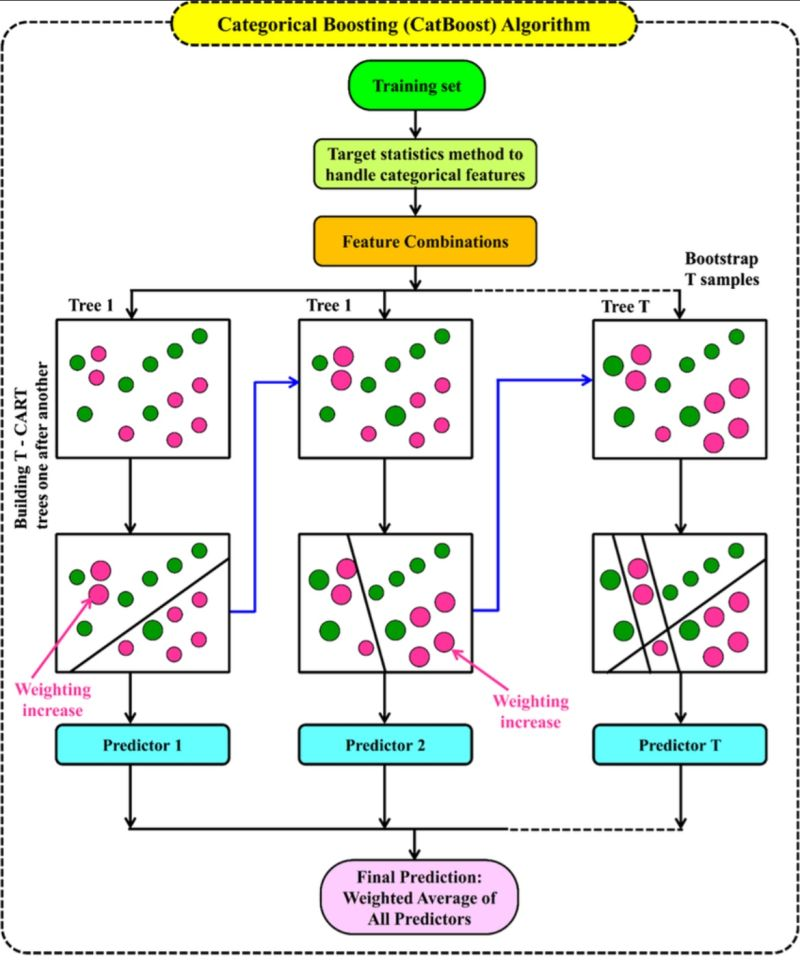
\includegraphics[width=0.7\linewidth]{images/catboost}
	\caption{مدل تقویت دسته‌ای}
	\label{fig:catboost}
\end{figure}


\subsection[شبکه عصبی چندلایه]{شبکه عصبی چندلایه\LTRfootnote{Multilayer Perceptrons (MLPs)}}


شبکه‌های عصبی در قلب بسیاری از الگوریتم‌ها و کاربردهای نوین یادگیری ماشین و هوش مصنوعی قرار دارند. در میان انواع مختلف این مدل‌ها، \textbf{ادراک‌گر چندلایه} یا \textbf{شبکه عصبی چندلایه} به‌عنوان یکی از اجزای پایه‌ای در یادگیری عمیق\LTRfootnote{Deep Learning} شناخته می‌شود. در این بخش، مفهوم شبکه عصبی مصنوعی معرفی می‌گردد و نحوه عملکرد ساختار چندلایه آن، شامل اجزایی مانند \textbf{انتشار رو‌به‌جلو}\LTRfootnote{Feedforward Propagation} و \textbf{پس‌انتشار خطا}\LTRfootnote{Backpropagation}  مورد بررسی قرار می‌گیرد.

\subsection*{مقدمه‌ای بر شبکه عصبی مصنوعی}

شبکه عصبی مصنوعی، یک مدل یادگیری ماشین است که ساختار آن الهام‌گرفته از ساختار و عملکرد شبکه نورون‌های درهم‌تنیده در مغز انسان می‌باشد. این شبکه از گره‌هایی موسوم به \textbf{نورون مصنوعی}\LTRfootnote{Artificial Neuron} تشکیل شده که در قالب لایه‌هایی به هم متصل هستند. جریان اطلاعات درون شبکه به‌گونه‌ای است که هر نورون، سیگنال ورودی را پردازش کرده و یک سیگنال خروجی تولید می‌کند که این خروجی می‌تواند به‌عنوان ورودی به نورون‌های بعدی منتقل شود.

\subsection*{ادراک‌گر چندلایه}

ادراک‌گر چندلایه، گونه‌ای از شبکه عصبی مصنوعی است که از چندین لایه از نورون‌ها تشکیل شده است. نورون‌های این ساختار معمولاً از \textbf{توابع فعال‌سازی}\LTRfootnote{Activation Functions} غیرخطی استفاده می‌کنند؛ امری که موجب توانایی یادگیری الگوهای پیچیده و غیرداده‌خطی در داده‌ها می‌شود. اهمیت این ساختار در یادگیری ماشین از آن‌جاست که می‌تواند روابط غیرخطی میان ویژگی‌ها و خروجی را مدل کند و در نتیجه برای وظایفی مانند دسته‌بندی، رگرسیون و شناسایی الگوها بسیار مؤثر است.

\subsection*{مبانی شبکه‌های عصبی}

شبکه‌های عصبی مصنوعی ابزارهای بنیادی در یادگیری ماشین محسوب می‌شوند و زیربنای بسیاری از الگوریتم‌ها و کاربردهای پیشرفته در حوزه‌هایی نظیر بینایی رایانه‌ای، پردازش زبان طبیعی، رباتیک و... را تشکیل می‌دهند.

هر شبکه از نورون‌هایی تشکیل شده که در لایه‌های مختلف سازمان‌دهی شده‌اند. هر نورون سیگنال‌های ورودی را دریافت کرده، با استفاده از یک تابع فعال‌سازی بر روی آن‌ها محاسبه انجام می‌دهد، و سیگنال خروجی تولید می‌کند. این توابع فعال‌سازی خروجی هر نورون را تعیین می‌کنند و با وارد کردن خاصیت غیرخطی به مدل، آن را قادر می‌سازند تا الگوهای پیچیده را فراگیرد.

ساختار شبکه معمولاً به‌صورت لایه‌ای تنظیم می‌شود؛ لایهٔ \textbf{ورودی} داده‌ها را دریافت می‌کند، سپس چندین لایه \textbf{میانی} (پنهان) عملیات محاسباتی را انجام می‌دهند، و نهایتاً \textbf{لایه خروجی} وظیفهٔ تولید پیش‌بینی یا تصمیم نهایی را بر عهده دارد.

اتصالات بین نورون‌های لایه‌های مجاور با وزن‌هایی مشخص تعریف می‌شوند که شدت تأثیر یک نورون بر نورون دیگر را نشان می‌دهند. این وزن‌ها در طول فرآیند آموزش و بر اساس داده‌های آموزشی تنظیم می‌گردند. همچنین، هر نورون معمولاً دارای یک \textbf{بایاس}\LTRfootnote{Bias} نیز هست که به تنظیم آستانهٔ خروجی نورون کمک می‌کند.

\subsection*{آموزش شبکه عصبی}

آموزش شبکه عصبی از طریق ترکیبی از انتشار روبه‌جلو و پس‌انتشار خطا صورت می‌گیرد. در مرحلهٔ انتشار روبه‌جلو، دادهٔ ورودی به‌صورت لایه‌به‌لایه از طریق شبکه عبور داده شده و هر لایه محاسبات لازم را انجام داده و خروجی را به لایهٔ بعدی ارسال می‌کند.

الگوریتم پس‌انتشار خطا به‌عنوان روش آموزش، وظیفه تنظیم وزن‌ها و بایاس‌ها را به‌عهده دارد. این الگوریتم با محاسبهٔ تابع زیان\LTRfootnote{Loss Function} که معیاری از اختلاف بین خروجی مدل و مقدار واقعی هدف است، مقدار خطا را در لایه خروجی محاسبه کرده و سپس آن را به‌صورت معکوس از خروجی به ورودی منتقل می‌کند تا تأثیر هر وزن بر خطا مشخص شود.

هدف آموزش، کمینه‌سازی مقدار تابع زیان است. این کار با استفاده از الگوریتم‌های بهینه‌سازی مانند نزول گرادیان انجام می‌گیرد که طی آن وزن‌ها و بایاس‌ها در جهت کاهش خطا به‌روزرسانی می‌شوند. در آموزش‌های با مجموعه داده‌های بزرگ، اغلب از روش \textbf{نزول گرادیان تصادفی} برای افزایش سرعت آموزش استفاده می‌شود.

در ادامه، برخی از این مفاهیم مانند توابع فعال‌سازی و ساختار لایه‌ها به‌تفصیل بررسی خواهند شد.

\subsection*{انواع شبکه‌های عصبی مصنوعی}

\begin{figure}[H]
	\centering
	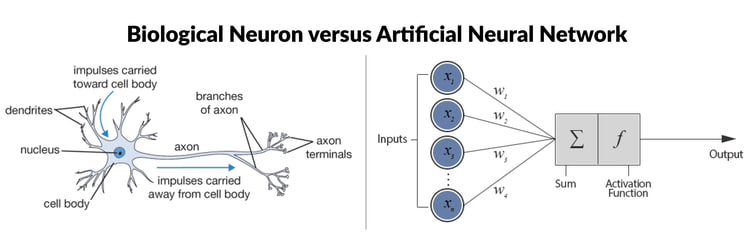
\includegraphics[width=0.7\linewidth]{images/Types_of_neuralnetwork}
	\caption{شبکه عصبی مصنوعی در مقابل شبکه عصبی بیولوژیکی}
	\label{fig:typesofneuralnetwork}
\end{figure}


مدلی که در سمت راست تصویر مشاهده می‌شود، یک شبکه عصبی ساده موسوم به \textbf{ادراک‌گر}\LTRfootnote{Perceptron} است. این مدل تنها از یک لایه تشکیل شده که همان لایهٔ ورودی است و شامل چندین نورون با وزن‌های مستقل می‌باشد. در این ساختار، هیچ لایهٔ میانی (پنهان) وجود ندارد. الگوریتم ادراک‌گر می‌کوشد وزن‌های سیگنال‌های ورودی را به‌گونه‌ای بیاموزد که یک مرز تصمیم‌گیری خطی میان داده‌ها ترسیم نماید.

با این حال، برای حل مسائل پیچیده‌تر و غیرداده‌خطی مانند پردازش تصویر، بینایی رایانه‌ای و پردازش زبان طبیعی، از شبکه‌های عصبی عمیق استفاده می‌شود.

شبکه‌های عصبی مصنوعی انواع مختلفی دارند که هر یک برای وظایف خاص و ساختارهای معماری متفاوت طراحی شده‌اند. در ادامه، برخی از رایج‌ترین انواع این شبکه‌ها معرفی می‌گردند:

\begin{enumerate}
	\item \textbf{شبکه‌های عصبی پیش‌خور}\LTRfootnote{Feedforward Neural Networks}
	
	این نوع از ساده‌ترین ساختارهای شبکه عصبی است که در آن اطلاعات تنها در یک جهت، از لایهٔ ورودی به لایهٔ خروجی جریان می‌یابد و هیچ‌گونه چرخه یا بازخوردی در ساختار آن وجود ندارد. مدل \textbf{ادراک‌گر چندلایه} نیز زیرمجموعه‌ای از این دسته محسوب می‌شود.
	
	\item \textbf{شبکه‌های عصبی بازگشتی}\LTRfootnote{Recurrent Neural Networks}
	
	در این شبکه‌ها، ارتباطات بین نورون‌ها به‌صورت چرخه‌ای و جهت‌دار طراحی می‌شوند تا اطلاعات در طول زمان حفظ شود. این ویژگی آن‌ها را برای مسائل داده‌های ترتیبی مانند پیش‌بینی سری‌های زمانی، پردازش زبان طبیعی و تشخیص گفتار مناسب می‌سازد.
	
	\item \textbf{شبکه‌های عصبی پیچشی}\LTRfootnote{Convolutional Neural Networks}
	
	این شبکه‌ها برای پردازش داده‌هایی با ساختار شبکه‌ای نظیر تصاویر طراحی شده‌اند. ساختار آن‌ها شامل لایه‌هایی از فیلترهای پیچشی است که ویژگی‌های داده را به‌صورت سلسله‌مراتبی استخراج می‌کنند. کاربردهای اصلی آن‌ها در طبقه‌بندی تصویر، شناسایی اشیاء و بخش‌بندی تصویر می‌باشد.
	
	\item \textbf{حافظهٔ بلندمدت کوتاه‌مدت}\LTRfootnote{Long Short-Term Memory Networks} و \textbf{واحدهای بازگشتی دروازه‌دار}\LTRfootnote{Gated Recurrent Units}
	
	این مدل‌ها نسخه‌های پیشرفته‌تری از شبکه‌های بازگشتی هستند که به‌منظور مقابله با مشکل ناپدید شدن گرادیان در شبکه‌های عصبی بازگشتی سنتی طراحی شده‌اند. استفاده از مکانیزم‌های دروازه‌ای در ساختار آن‌ها موجب توانایی در یادگیری وابستگی‌های بلندمدت در داده‌های ترتیبی شده و در وظایفی مانند ترجمه ماشینی، تشخیص احساسات و تشخیص گفتار بسیار کارآمد هستند.
	
	\item \textbf{خودرمزگذارها}\LTRfootnote{Autoencoders}
	
	این مدل‌ها برای یادگیری بدون ناظر طراحی شده‌اند و از دو بخش تشکیل می‌شوند: بخش \textbf{رمزگذار} که دادهٔ ورودی را به یک فضای نهفته با ابعاد کمتر فشرده می‌کند، و بخش \textbf{بازرمزگذار} که از روی فضای نهفته تلاش می‌کند ورودی اولیه را بازسازی نماید. کاربردهای اصلی آن‌ها شامل کاهش ابعاد، حذف نویز از داده و مدل‌سازی مولد است.
	
	\item \textbf{شبکه‌های مولد تخاصمی}\LTRfootnote{Generative Adversarial Networks}
	
	این ساختار شامل دو شبکهٔ عصبی است: یک \textbf{تولیدکننده} و یک \textbf{تمایزدهنده} که به‌صورت رقابتی آموزش می‌بینند. تولیدکننده می‌کوشد داده‌هایی مشابه داده‌های واقعی بسازد، در حالی که تمایزدهنده وظیفهٔ تشخیص داده‌های واقعی از داده‌های ساختگی را دارد. این شبکه‌ها در تولید تصاویر واقع‌گرایانه، ویدیوها و انواع دیگر داده بسیار موفق بوده‌اند.
\end{enumerate}


\subsection*{ادراک‌گر چندلایه}

ادراک‌گر چندلایه یک نوع از \textbf{شبکه عصبی پیش‌خور} است که از نورون‌هایی کاملاً متصل به یکدیگر تشکیل شده و از توابع فعال‌سازی غیرخطی\LTRfootnote{Nonlinear Activation Function} بهره می‌برد. این مدل به‌طور گسترده برای تفکیک داده‌هایی که به‌صورت خطی جداپذیر نیستند مورد استفاده قرار می‌گیرد.

ادراک‌گرهای چندلایه کاربردهای فراوانی در حوزه‌هایی چون شناسایی تصویر، پردازش زبان طبیعی و تشخیص گفتار دارند. انعطاف‌پذیری معماری و توانایی آن‌ها در تقریب هر تابعی (تحت شرایط خاص) سبب شده که از آن‌ها به‌عنوان اجزای بنیادی در یادگیری عمیق و پژوهش‌های مرتبط با شبکه‌های عصبی یاد شود. در ادامه به بررسی اجزای اصلی این ساختار پرداخته می‌شود:

\paragraph{لایه ورودی:}
لایهٔ ورودی از نورون‌هایی تشکیل شده که داده‌های خام اولیه را دریافت می‌کنند. هر نورون در این لایه معرف یکی از ویژگی‌ها یا ابعاد دادهٔ ورودی است. تعداد نورون‌های این لایه برابر با تعداد ویژگی‌های مسئله است.

\paragraph{لایه میانی (پنهان):}
بین لایهٔ ورودی و خروجی، یک یا چند \textbf{لایه میانی}\LTRfootnote{Hidden Layer} وجود دارد. هر نورون در یک لایه میانی، ورودی‌هایی از تمام نورون‌های لایهٔ قبلی دریافت کرده و خروجی‌ای تولید می‌کند که به لایهٔ بعدی منتقل می‌شود. تعداد این لایه‌ها و تعداد نورون‌ها در هر لایه از جمله فراپارامترها\LTRfootnote{Hyperparameters} محسوب می‌شود که در مرحلهٔ طراحی مدل مشخص می‌گردند.

\paragraph{لایه خروجی:}
این لایه شامل نورون‌هایی است که خروجی نهایی شبکه را تولید می‌کنند. تعداد نورون‌های این لایه به ماهیت مسئله بستگی دارد. برای مثال، در دسته‌بندی دودویی ممکن است یک یا دو نورون وجود داشته باشد که احتمال تعلق نمونه به یک رده را نمایش دهند. در مسائل دسته‌بندی چندرده‌ای، تعداد نورون‌ها برابر با تعداد کلاس‌ها خواهد بود.

\paragraph{وزن‌ها:}
اتصالات بین نورون‌های لایه‌های متوالی با وزن‌هایی\LTRfootnote{Weights} مشخص تعریف می‌شوند که شدت تأثیر یک نورون بر نورون بعدی را تعیین می‌کنند. این وزن‌ها طی فرآیند آموزش به‌روز می‌شوند تا مدل بتواند به‌درستی الگوهای موجود در داده را بیاموزد.

\paragraph{نورون‌های بایاس:}
در اغلب ساختارها، هر لایه (به‌جز لایهٔ ورودی) دارای یک \textbf{نورون بایاس}\LTRfootnote{Bias Neuron} است که مقدار ثابتی را به نورون‌های لایهٔ بعدی ارسال می‌کند. بایاس‌ها نیز دارای وزن مخصوص به خود هستند و در طول آموزش مدل یاد گرفته می‌شوند. وجود این نورون‌ها باعث می‌شود تابع فعال‌سازی نورون‌های بعدی جابه‌جا شده و مدل قادر به یادگیری شیفت یا بایاس در مرز تصمیم‌گیری باشد.

\textit{نکته}: در فضای یادگیری ماشین، اصطلاح «بایاس» می‌تواند به دو مفهوم مرتبط ولی متمایز اشاره کند: یکی بایاس به‌عنوان نورون در ساختار شبکه، و دیگری \textbf{سوگیری مدل}\LTRfootnote{Model Bias} که به میزان ساده‌سازی مدل در تخمین واقعیت اشاره دارد. سوگیری زیاد نشان‌دهندهٔ مدلی ساده‌انگار و دارای \textbf{کم‌برازش} است، در حالی که سوگیری کم بیانگر قدرت بیشتر مدل در یادگیری الگوهای پنهان داده است.

\paragraph{توابع فعال‌سازی:}
معمولاً هر نورون در لایه‌های میانی و خروجی از یک تابع فعال‌سازی برای اعمال بر مجموع وزنی ورودی‌های خود استفاده می‌کند. توابع رایج در این زمینه شامل \textbf{سیگموید}\LTRfootnote{Sigmoid}، \textbf{تانژانت}\LTRfootnote{Tanh}، \textbf{واحد خطی اصلاح‌شده}\LTRfootnote{Rectified Linear Unit (ReLU)} و \textbf{سافت‌مکس}\LTRfootnote{Softmax} هستند. وجود این توابع موجب غیرخطی شدن مدل شده و قابلیت یادگیری الگوهای پیچیده‌تر را فراهم می‌کند.

\paragraph{انتشار روبه‌جلو و پس‌انتشار خطا:}
آموزش ادراک‌گر چندلایه با استفاده از الگوریتم \textbf{پس‌انتشار خطا} صورت می‌گیرد. در این روش، ابتدا در مرحله \textbf{انتشار روبه‌جلو}، داده از لایه ورودی به لایه خروجی منتقل شده و خروجی مدل محاسبه می‌شود. سپس با محاسبه تابع زیان، میزان خطای مدل سنجیده می‌شود. در مرحلهٔ بعد، گرادیان تابع زیان نسبت به وزن‌ها محاسبه شده و با استفاده از الگوریتمی نظیر نزول گرادیان، وزن‌ها به‌روزرسانی می‌شوند تا تابع زیان به‌مرور کمینه گردد.


\subsection*{عملکرد شبکه عصبی چندلایه به‌صورت گام‌به‌گام}

\begin{figure}[H]
	\centering
	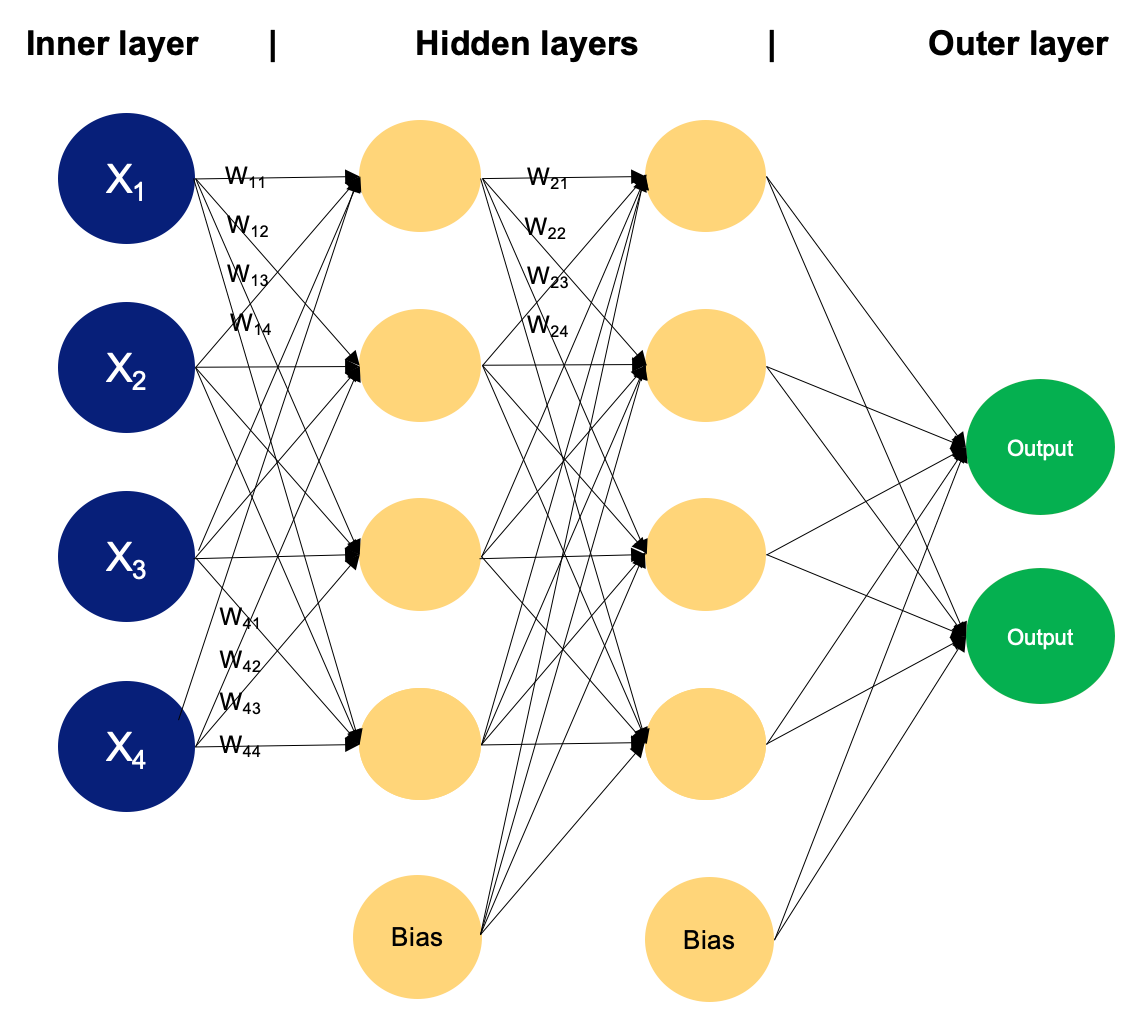
\includegraphics[width=0.7\linewidth]{images/MLP}
	\caption{ساختار شبکه‌های عصبی چندلایه}
	\label{fig:mlp}
\end{figure}


در یک شبکه عصبی چندلایه، نورون‌ها به‌صورت مرحله‌به‌مرحله اطلاعات را پردازش می‌کنند. در هر مرحله محاسباتی شامل جمع وزنی ورودی‌ها و تبدیل‌های غیرخطی انجام می‌شود. در ادامه، به بررسی عملکرد این مدل به‌صورت لایه به لایه پرداخته می‌شود:

\paragraph{لایه ورودی:}
لایهٔ ورودی، داده‌های اولیه (ویژگی‌های استخراج‌شده از نمونه‌های مجموعه داده) را دریافت می‌کند. هر نورون در این لایه نمایندهٔ یک ویژگی از داده است. نورون‌های لایهٔ ورودی هیچ‌گونه پردازشی روی داده انجام نمی‌دهند و صرفاً مقادیر ورودی را به لایهٔ میانی اول منتقل می‌کنند.

\paragraph{لایه‌های میانی:}
در لایه‌های میانی، نورون‌ها با دریافت ورودی از نورون‌های لایهٔ قبلی، عملیات محاسباتی انجام می‌دهند. هر ورودی با وزن متناظر خود (نماد $w$) ضرب می‌شود. این وزن‌ها نشان می‌دهند که هر ورودی تا چه میزان بر خروجی نورون تأثیرگذار است. علاوه بر وزن، هر نورون دارای یک مقدار بایاس با نماد $b$ است که مانند یک ورودی اضافی به نورون عمل کرده و به تنظیم آستانه خروجی کمک می‌کند. وزن و بایاس هر دو در فرآیند آموزش مدل یاد گرفته می‌شوند.

برای هر نورون در لایهٔ میانی یا خروجی، مجموع وزنی ورودی‌ها به‌صورت زیر محاسبه می‌شود:
\[
\text{Weighted Sum} = \sum_{i=1}^{n} w_i x_i + b
\]

در این رابطه، $n$ تعداد کل ورودی‌ها، $x_i$ مقدار $i$-امین ورودی، و $w_i$ وزن متناظر آن است. این مقدار سپس از طریق یک تابع فعال‌سازی عبور داده می‌شود تا خروجی نهایی نورون تولید شود. این تابع با افزودن خاصیت غیرخطی، توانایی مدل در یادگیری الگوهای پیچیده را افزایش می‌دهد. انتخاب تابع فعال‌سازی به ماهیت مسئله و ویژگی‌های مورد انتظار مدل بستگی دارد.

\paragraph{لایه خروجی:}
لایهٔ خروجی وظیفهٔ تولید پیش‌بینی نهایی یا پاسخ مدل را دارد. تعداد نورون‌های این لایه با توجه به نوع مسئله تعیین می‌شود (مثلاً در دسته‌بندی دودویی یا چندرده‌ای یا در مسائل رگرسیون). هر نورون در این لایه از نورون‌های لایهٔ میانی قبلی ورودی گرفته و پس از اعمال تابع فعال‌سازی خروجی نهایی را تولید می‌کند. تابع فعال‌سازی در لایهٔ خروجی ممکن است با توابع استفاده‌شده در لایه‌های میانی متفاوت باشد.

در فرآیند آموزش، شبکه تلاش می‌کند با تنظیم وزن‌ها و بایاس‌ها، تفاوت بین خروجی پیش‌بینی‌شده و مقدار واقعی هدف را به حداقل برساند. این کار از طریق به‌روزرسانی پیوسته وزن‌ها بر اساس داده‌های آموزشی انجام می‌شود. به‌این‌ترتیب مدل قادر خواهد بود الگوهای پنهان در داده را فراگرفته و روی نمونه‌های جدید، پیش‌بینی دقیقی انجام دهد.

این بهینه‌سازی با استفاده از الگوریتم‌هایی نظیر نزول گرادیان تصادفی انجام می‌شود. در این الگوریتم، گرادیان تابع زیان نسبت به وزن‌ها محاسبه شده و وزن‌ها در جهت کاهش تابع زیان به‌روزرسانی می‌شوند.


\subsection[شبکه عصبی عمیق]{شبکه عصبی عمیق\LTRfootnote{Deep Neural Networks(DNN)}}

شبکه‌های عصبی عمیق مدل‌هایی هستند که با بهره‌گیری از ساختارهای لایه‌ای پیچیده، به ماشین‌ها امکان می‌دهند الگوها و نمایش‌های پیچیده‌ای را از داده‌ها بیاموزند. این شبکه‌ها در صورت آموزش مناسب، توانایی تفسیر دقیق تصاویر، تقلید گفتار انسان‌مانند، و حتی تولید آثار هنری را با دقت بالا برای مدل‌های یادگیری ماشین فراهم می‌سازند.

\subsection*{تعریف شبکه عصبی عمیق}

شبکه عصبی عمیق نوعی از شبکه‌های عصبی مصنوعی است که دارای چندین لایه بین لایه ورودی و خروجی می‌باشد. هر لایه شامل تعدادی گره محاسباتی است که عملیات پردازش را بر روی داده‌های ورودی انجام می‌دهند. نام دیگر این ساختار در ادبیات علمی، \textbf{شبکه عمیق} نیز می‌باشد.

اصطلاح عمیق در شبکه‌های عصبی عمیق به وجود چندین لایه پنهان اشاره دارد؛ این لایه‌ها موجب می‌شوند شبکه بتواند نمایش‌های پیچیده و سطح بالایی از داده‌های ورودی استخراج کند. در واقع همین ساختار چندلایه‌ای است که شبکه‌های عمیق را قادر می‌سازد تا مسائل پیچیده‌ای را حل کنند که توسط ساختارهای ساده‌تر و کم‌عمق‌تر قابل حل نیستند.

\begin{figure}[H]
	\centering
	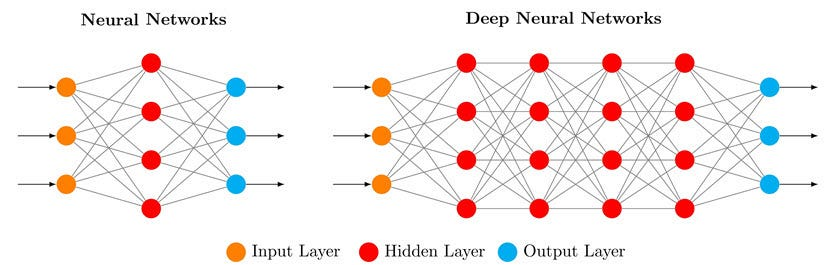
\includegraphics[width=0.7\linewidth]{images/dnn}
	\caption{شبکه‌های عصبی و شبکه‌های عصبی عمیق}
	\label{fig:dnn}
\end{figure}


لایه‌های پنهان در یک شبکه عصبی عمیق معمولاً از نوع لایه‌های متراکم (کامل متصل)\LTRfootnote{Dense (Fully Connected) Layers} هستند. در این ساختار، هر نورون در یک لایه پنهان به تمام نورون‌های لایهٔ قبلی و بعدی متصل است. این ویژگی موجب می‌شود شبکه‌های عصبی عمیق برای یادگیری روابط پیچیده در داده‌ها بسیار مناسب باشند.

نکتهٔ مهم آن است که لایه‌های پنهان در یک شبکه عصبی عمیق، صرفاً نسخه‌های تکراری از یکدیگر نیستند. در عوض، این شبکه‌ها دارای ساختارهای متنوع و پیچیده‌ای از لایه‌ها هستند که هرکدام نقشی خاص در یادگیری ایفا می‌کنند. برخی از انواع رایج لایه‌های مورد استفاده در این شبکه‌ها عبارت‌اند از:

\begin{itemize}
	\item \textbf{لایه‌های پیچشی}\LTRfootnote{Convolutional Layers} که مجموعه‌ای از فیلترهای قابل یادگیری را بر روی داده‌های ورودی اعمال می‌کنند.
	\item \textbf{لایه‌های حافظهٔ بلند کوتاه‌مدت}\LTRfootnote{Long Short-Term Memory (LSTM) Layers} که وابستگی‌های زمانی در داده‌های ترتیبی را استخراج می‌کنند.
	\item \textbf{واحدهای بازگشتی دروازه‌دار}\LTRfootnote{Gated Recurrent Unit (GRU) Layers} که با استفاده از مکانیزم دروازه‌ای جریان اطلاعات را در شبکه کنترل می‌کنند.
	\item \textbf{لایه‌های توجه}\LTRfootnote{Attention Layers} که در هنگام پیش‌بینی، تمرکز شبکه را بر بخش‌های خاصی از توالی ورودی معطوف می‌سازند.
	\item \textbf{لایه‌های نرمال‌سازی}\LTRfootnote{Normalization Layers} که موجب پایداری و تسریع فرآیند آموزش در شبکه می‌شوند.
\end{itemize}

هرچه تعداد لایه‌های پنهان در یک شبکه عصبی عمیق بیشتر باشد، توانایی آن در یادگیری و پردازش داده‌های ورودی نیز افزایش می‌یابد. گرچه شبکه‌ای که تنها دو لایه پنهان دارد نیز «عمیق» محسوب می‌شود، در عمل بسیاری از شبکه‌های عصبی عمیق دارای صدها لایهٔ پنهان میان ورودی و خروجی هستند.


\subsection*{نحوهٔ عملکرد شبکه‌های عصبی عمیق}

شبکه‌های عصبی عمیق از چندین لایه متشکل از گره‌هایی به نام نورون‌ یا واحد تشکیل شده‌اند. این شبکه‌ها معمولاً شامل سه نوع لایه هستند:

\begin{itemize}
	\item \textbf{لایهٔ ورودی:} وظیفهٔ دریافت داده‌های خام را برعهده دارد. هر نورون در این لایه نمایانگر یک ویژگی از دادهٔ ورودی است. به عنوان نمونه، برای تفسیر تصاویری با ابعاد \lr{28×28} پیکسل، به \lr{784} نورون در لایهٔ ورودی نیاز است؛ زیرا هر نورون نشان‌دهندهٔ شدت روشنایی یک پیکسل با مقداری در بازهٔ \lr{0} تا \lr{255} است.
	
	\item \textbf{لایه‌های پنهان:} این لایه‌ها بین لایهٔ ورودی و لایهٔ خروجی قرار دارند و معمولاً بیش از دو عدد هستند. هر لایهٔ پنهان از چندین نورون تشکیل شده است که به نورون‌های لایه‌های مجاور متصل‌اند، اما نورون‌های یک لایه به یکدیگر متصل نمی‌باشند.
	
	\item \textbf{لایهٔ خروجی:} این لایه مسئول تولید خروجی نهایی شبکه است. تعداد نورون‌های این لایه بسته به نوع مسئله (مانند طبقه‌بندی دودویی، چندکلاسه یا رگرسیون) تعیین می‌شود.
\end{itemize}

پس از وارد شدن داده‌های خام، این داده‌ها به‌صورت لایه‌به‌لایه از طریق شبکه به جلو هدایت می‌شوند. در هر لایه، نورون‌ها ابتدا با استفاده از تابع فعال‌سازی اختصاص‌یافته، بر ورودی‌ها عملیات پردازشی انجام داده و سپس خروجی پردازش‌شده را به لایهٔ بعدی ارسال می‌کنند.

در ادامه، چند تابع فعال‌سازی رایج معرفی می‌شود:

\begin{itemize}
	\item \textbf{سیگموئید}\LTRfootnote{Sigmoid}: مقدار ورودی را در بازهٔ 0 تا 1 فشرده‌سازی می‌کند و برای مسائل طبقه‌بندی دودویی مناسب است.
	
	\item \textbf{تانژانت هاپربولیک}\LTRfootnote{Hyperbolic Tangent (Tanh)}: ورودی را در بازهٔ -1 تا 1 نگاشت می‌کند و در مسائل طبقه‌بندی و رگرسیون کاربرد دارد.
	
	\item \textbf{واحد خطی اصلاح‌شده}\LTRfootnote{Rectified Linear Unit (ReLU)}: مقادیر منفی ورودی را صفر و مقادیر مثبت را بدون تغییر عبور می‌دهد.
	
	\item \textbf{تابع سافت‌مکس}\LTRfootnote{Softmax Function}: امتیازهای خام را به مقادیر احتمالی تبدیل می‌کند، به‌طوری‌که مجموع خروجی‌ها برابر با 1 باشد.
\end{itemize}

پس از تولید خروجی نهایی توسط شبکه، این خروجی با مقدار هدف که از سوی طراح یا کاربر تعیین شده مقایسه می‌شود. اختلاف میان مقدار پیش‌بینی‌شده و مقدار واقعی توسط تابع هدف یا تابع زیان سنجیده می‌شود. سپس این خطاها به‌صورت معکوس در شبکه منتشر شده و وزن‌های ارتباطی نورون‌ها با استفاده از الگوریتم‌های بهینه‌سازی، به‌گونه‌ای تنظیم می‌گردند که مقدار خطا کاهش یابد.

\subsection*{شبکه‌های عصبی و مفهوم وزن‌دهی}

در یک شبکهٔ عصبی عمیق، هر اتصال بین نورون‌های دو لایهٔ مجاور دارای یک وزن عددی است. این وزن‌ها بیانگر \textbf{قدرت تأثیرگذاری} خروجی یک نورون بر ورودی نورون دیگر می‌باشند و میزان اهمیت یا نفوذ یک نورون را در فرآیند انتقال اطلاعات مشخص می‌کنند.

وزن‌ها می‌توانند دارای مقادیر مثبت یا منفی باشند که نوع و شدت اثر نورون‌ها بر یکدیگر را تعیین می‌کند:

\begin{itemize}
	\item \textbf{وزن مثبت:} اگر وزنی مثبت باشد، افزایش در خروجی نورون مبدأ منجر به افزایش فعالیت نورون مقصد خواهد شد. در این حالت، نورون مبدأ فعالیت نورون مقصد را \textbf{تحریک} می‌کند.
	
	\item \textbf{وزن منفی:} در صورتی‌که وزن منفی باشد، افزایش در خروجی نورون مبدأ منجر به کاهش فعالیت نورون مقصد می‌شود. در این حالت، نورون مبدأ فعالیت نورون مقصد را \textbf{مهار} می‌کند.
\end{itemize}

در ابتدای آموزش، وزن‌های شبکه معمولاً به‌صورت تصادفی مقداردهی اولیه می‌شوند. سپس در طول فرایند آموزش، شبکهٔ عصبی این وزن‌ها را به‌طور تدریجی و تکرارشونده بر اساس تفاوت میان خروجی پیش‌بینی‌شده و مقدار واقعی به‌روزرسانی می‌کند.

وزن‌ها نقش بسیار حیاتی در هر دو مرحلهٔ \textbf{انتشار} و \textbf{پس انتشار} در شبکه‌های عمیق ایفا می‌کنند:

\begin{itemize}
	\item در مرحلهٔ \textbf{انتشار}، هر نورون مجموع وزن‌دار ورودی‌های خود را از نورون‌های لایهٔ قبل محاسبه کرده و سپس با اعمال یک تابع فعال‌سازی بر این مجموع، خروجی خود را تولید و به لایهٔ بعدی ارسال می‌کند.
	
	\item در مرحلهٔ \textbf{پس‌انتشار}، سیگنال خطا از خروجی شبکه به‌صورت معکوس در لایه‌ها انتشار می‌یابد. در این فرآیند، وزن‌ها به گونه‌ای تنظیم می‌شوند که مقدار خطا کاهش یابد.
\end{itemize}

بهینه‌سازی وزن‌ها از اجزای کلیدی در آموزش شبکه‌های عصبی است، زیرا تعیین می‌کند که شبکه تا چه حد قادر به یادگیری الگوهای معنادار از داده‌های آموزشی و تولید پیش‌بینی‌های دقیق باشد.


\subsection*{چالش‌های شبکه‌های عصبی عمیق}

اگرچه شبکه‌های عصبی عمیق توانایی‌های چشمگیری در یادگیری الگوهای پیچیده دارند، اما استفاده از آن‌ها با چالش‌هایی همراه است که آگاهی از آن‌ها پیش از آغاز فرایند آموزش ضروری است. در ادامه، مهم‌ترین مشکلاتی که در پیاده‌سازی و آموزش این مدل‌ها ممکن است رخ دهد بررسی می‌گردد.

\subsection*{کیفیت و کمیت داده‌های آموزشی}

برای آموزش مناسب یک شبکهٔ عصبی عمیق و تضمین تعمیم‌پذیری آن نسبت به ورودی‌های جدید و دیده‌نشده، به حجم بالایی از داده‌های برچسب‌خوردهٔ دقیق نیاز است. تهیهٔ این داده‌ها به‌ویژه در حوزه‌هایی که فرایند برچسب‌گذاری دشوار یا پرهزینه است، زمان‌بر و پرهزینه می‌باشد.

داده‌هایی که به لایهٔ ورودی شبکه تزریق می‌شوند باید دارای ویژگی‌های زیر باشند:

\begin{itemize}
	\item \textbf{دقت:} وجود خطا در برچسب‌ها یا داده‌های نادقیق منجر به یادگیری الگوهای نادرست و پیش‌بینی‌های اشتباه توسط مدل می‌شود.
	\item \textbf{نمایندگی:\LTRfootnote{Representativeness}} داده‌های آموزشی باید تمام حالات و تنوع‌های ممکن را که مدل در محیط واقعی با آن مواجه خواهد شد پوشش دهند؛ در غیر این‌صورت، مدل دچار سوگیری یا پیش‌بینی ناقص خواهد شد.
	\item \textbf{پاکی:\LTRfootnote{Cleanness}} وجود نویز یا نقاط پرت در داده‌ها باعث ایجاد ابهام در فرایند یادگیری و کاهش عملکرد مدل می‌شود.
\end{itemize}

بهبود کیفیت و کمیت داده‌های آموزشی مستلزم جمع‌آوری اصولی، برچسب‌گذاری دقیق، پیش‌پردازش مناسب و اعتبارسنجی داده‌هاست. همچنین استفاده از تکنیک‌های افزایش داده، مانند چرخش، تغییر اندازه، برش، یا افزودن نویز می‌تواند موجب افزایش حجم مؤثر داده‌ها شود.

\subsection*{چالش‌های آموزش شبکه}

دو چالش اصلی در آموزش شبکه‌های عصبی عمیق، بیش‌برازش و کم‌برازش هستند که بر توانایی مدل در تعمیم به داده‌های جدید تأثیر می‌گذارند.

\paragraph{بیش‌برازش:} زمانی رخ می‌دهد که مدل به‌جای یادگیری روابط بنیادین میان ویژگی‌ها، جزئیات خاص و نویز موجود در داده‌های آموزشی را حفظ می‌کند. نتیجهٔ این حالت، عملکرد بسیار خوب مدل روی داده‌های آموزش و عملکرد ضعیف آن روی داده‌های جدید است.

نشانه‌های بیش‌برازش شامل دقت بالای آموزش، دقت پایین اعتبارسنجی و نمودارهای نوسانی یا نامنظم در روند آموزش است. برای مقابله با این مشکل، روش‌های زیر توصیه می‌شود:

\begin{itemize}
	\item استفاده از منظم‌سازی، حذف تصادفی نورون‌ها\LTRfootnote{Dropout} و توقف زودهنگام در حین آموزش،
	\item افزایش تنوع و حجم داده‌ها از طریق تکنیک‌های افزایش داده،
	\item کاهش پیچیدگی مدل با کاهش عمق یا عرض شبکه.
\end{itemize}

\paragraph{کم‌برازش:} زمانی رخ می‌دهد که مدل ساختار بسیار ساده‌ای دارد و قادر به یادگیری روابط اساسی میان ویژگی‌ها نیست. این مشکل موجب عملکرد ضعیف هم در داده‌های آموزش و هم در اعتبارسنجی می‌شود. برای حل این مشکل می‌توان:

\begin{itemize}
	\item افزایش پیچیدگی مدل از طریق افزایش تعداد لایه‌ها یا نورون‌ها،
	\item افزودن ویژگی‌های مؤثرتر به ورودی مدل،
	\item افزایش تنوع داده‌های آموزشی.
\end{itemize}

یکی دیگر از مشکلات رایج در آموزش این مدل‌ها، \textbf{ناپدید شدن گرادیان}\LTRfootnote{Vanishing Gradient} در طول فرایند انتشار معکوس است که باعث کندی یا توقف آموزش می‌شود.

\subsection*{تنظیم ابرپارامترها}

ابرپارامترها نقش حیاتی در تعیین رفتار و عملکرد شبکهٔ عصبی دارند. این پارامترها پیش از شروع آموزش تعریف می‌شوند و باید متناسب با هدف مدل انتخاب شوند. مهم‌ترین ابرپارامترها عبارت‌اند از:

\begin{itemize}
	\item نرخ یادگیری،
	\item اندازهٔ دسته‌های آموزشی،
	\item تعداد لایه‌ها،
	\item تعداد نورون‌ها در هر لایه،
	\item میزان منظم‌سازی،
	\item نرخ حذف نورون‌ها،
	\item نوع توابع فعال‌سازی،
	\item الگوریتم‌های بهینه‌سازی.
\end{itemize}

تنظیم نادرست این پارامترها می‌تواند منجر به آموزش کند، عملکرد ضعیف، و تعمیم‌پذیری پایین شود. از آنجا که این ابرپارامترها اثر متقابل و پیچیده‌ای بر یکدیگر دارند، تعیین پیکربندی بهینه معمولاً از طریق آزمون و خطا و تحلیل دقیق شاخص‌های آموزش انجام می‌گیرد که نیازمند زمان و دقت فراوان است.





\section{معیارهای ارزیابی مدل‌ها}

برای ارزیابی مدل‌های پیش‌بینی، از شش شاخص اصلی استفاده شده است:

\begin{enumerate}
	\item \textbf{ضریب تعیین}
\[
R^2 = 1 - \frac{\sum_{i}(y_i - \hat{y}_i)^2}{\sum_{i}(y_i - \bar{y})^2}
\]
نشان‌دهنده درصد واریانس توضیح داده‌شده توسط مدل.

	\item \textbf{میانگین قدرمطلق خطا}
\[
MAE = \frac{1}{n} \sum_{i=1}^{n} |y_i - \hat{y}_i|
\]
مقدار میانگین قدرمطلق خطا بین پیش‌بینی و مقدار واقعی.

	\item \textbf{ریشه میانگین مربع خطا}
\[
RMSE = \sqrt{ \frac{1}{n} \sum_{i=1}^{n} (y_i - \hat{y}_i)^2 }
\]
شاخصی حساس به خطاهای بزرگ.

	\item \textbf{درصد خطای میانگین}
\[
MPE = \frac{100}{n} \sum_{i=1}^{n} \frac{y_i - \hat{y}_i}{y_i}
\]
برای بررسی جهت کلی خطا.

	\item \textbf{میانگین قدرمطلق درصد خطای متقارن}
\[
sMAPE = \frac{100}{n} \sum_{i=1}^{n} \frac{|y_i - \hat{y}_i|}{(|y_i| + |\hat{y}_i|)/2}
\]
مناسب برای مقایسه مقادیر نسبی خطا.

	\item \textbf{انحراف استاندارد نسبی}
\[
SDR = \frac{RMSE}{\sigma_y}
\]
که \(\sigma_y\) انحراف معیار مشاهدات واقعی است. این شاخص میزان پراکندگی خطا نسبت به پراکندگی داده‌ها را نشان می‌دهد.
\end{enumerate}
